% Options for packages loaded elsewhere
\PassOptionsToPackage{unicode}{hyperref}
\PassOptionsToPackage{hyphens}{url}
%
\documentclass[
]{article}
\usepackage{amsmath,amssymb}
\usepackage{lmodern}
\usepackage{ifxetex,ifluatex}
\ifnum 0\ifxetex 1\fi\ifluatex 1\fi=0 % if pdftex
  \usepackage[T1]{fontenc}
  \usepackage[utf8]{inputenc}
  \usepackage{textcomp} % provide euro and other symbols
\else % if luatex or xetex
  \usepackage{unicode-math}
  \defaultfontfeatures{Scale=MatchLowercase}
  \defaultfontfeatures[\rmfamily]{Ligatures=TeX,Scale=1}
\fi
% Use upquote if available, for straight quotes in verbatim environments
\IfFileExists{upquote.sty}{\usepackage{upquote}}{}
\IfFileExists{microtype.sty}{% use microtype if available
  \usepackage[]{microtype}
  \UseMicrotypeSet[protrusion]{basicmath} % disable protrusion for tt fonts
}{}
\makeatletter
\@ifundefined{KOMAClassName}{% if non-KOMA class
  \IfFileExists{parskip.sty}{%
    \usepackage{parskip}
  }{% else
    \setlength{\parindent}{0pt}
    \setlength{\parskip}{6pt plus 2pt minus 1pt}}
}{% if KOMA class
  \KOMAoptions{parskip=half}}
\makeatother
\usepackage{xcolor}
\IfFileExists{xurl.sty}{\usepackage{xurl}}{} % add URL line breaks if available
\IfFileExists{bookmark.sty}{\usepackage{bookmark}}{\usepackage{hyperref}}
\hypersetup{
  pdftitle={Text Mining Analysis of the best-seller non-fiction book: Invisible Women, by Caroline Perez Criado},
  pdfauthor={Aëllya Monney, Colin Steffe, Rémy Tombola and Jasmine Mawjee},
  hidelinks,
  pdfcreator={LaTeX via pandoc}}
\urlstyle{same} % disable monospaced font for URLs
\usepackage[margin=1in]{geometry}
\usepackage{longtable,booktabs,array}
\usepackage{calc} % for calculating minipage widths
% Correct order of tables after \paragraph or \subparagraph
\usepackage{etoolbox}
\makeatletter
\patchcmd\longtable{\par}{\if@noskipsec\mbox{}\fi\par}{}{}
\makeatother
% Allow footnotes in longtable head/foot
\IfFileExists{footnotehyper.sty}{\usepackage{footnotehyper}}{\usepackage{footnote}}
\makesavenoteenv{longtable}
\usepackage{graphicx}
\makeatletter
\def\maxwidth{\ifdim\Gin@nat@width>\linewidth\linewidth\else\Gin@nat@width\fi}
\def\maxheight{\ifdim\Gin@nat@height>\textheight\textheight\else\Gin@nat@height\fi}
\makeatother
% Scale images if necessary, so that they will not overflow the page
% margins by default, and it is still possible to overwrite the defaults
% using explicit options in \includegraphics[width, height, ...]{}
\setkeys{Gin}{width=\maxwidth,height=\maxheight,keepaspectratio}
% Set default figure placement to htbp
\makeatletter
\def\fps@figure{htbp}
\makeatother
\setlength{\emergencystretch}{3em} % prevent overfull lines
\providecommand{\tightlist}{%
  \setlength{\itemsep}{0pt}\setlength{\parskip}{0pt}}
\setcounter{secnumdepth}{-\maxdimen} % remove section numbering
\usepackage{booktabs}
\usepackage{longtable}
\usepackage{array}
\usepackage{multirow}
\usepackage{wrapfig}
\usepackage{float}
\usepackage{colortbl}
\usepackage{pdflscape}
\usepackage{tabu}
\usepackage{threeparttable}
\usepackage{threeparttablex}
\usepackage[normalem]{ulem}
\usepackage{makecell}
\usepackage{xcolor}
\ifluatex
  \usepackage{selnolig}  % disable illegal ligatures
\fi

\title{Text Mining Analysis of the best-seller non-fiction book:
Invisible Women, by Caroline Perez Criado}
\author{Aëllya Monney, Colin Steffe, Rémy Tombola and Jasmine Mawjee}
\date{13 décembre, 2021}

\begin{document}
\maketitle

\hypertarget{executive-summary}{%
\section{Executive Summary}\label{executive-summary}}

This report outlines the results of a text mining analysis of the
best-seller non-fiction book \emph{Invisible Women}. Its exploration is
meant to better understand some textual characteristics of feminist
texts. Our text mining analysis shows that {[}ADD RESULTS HERE{]}.

\hypertarget{introduction}{%
\section{Introduction}\label{introduction}}

The goal of the analysis is to study textual data and extract some
specific characteristics of feminist texts on gender bias in data.

The upcoming analysis is a comprehensive text mining exploration of
\emph{Invisible Women} following a four-part structure:

\begin{itemize}
\tightlist
\item
  Data gathering
\item
  Cleaning and exploratory data analysis

  \begin{itemize}
  \tightlist
  \item
    Tokenization
  \item
    Stop Words
  \item
    Lemmatization
  \item
    Stemming
  \item
    Document-Term Matrix (DTM)
  \item
    Term Frequency and Inverse Document Matrix (TF-IDF)
  \item
    Zipf's Law
  \end{itemize}
\item
  Unsupervised analysis {[}ADD SUBSECTIONS{]}
\item
  Supervised learning {[}ADD SUBSECTIONS{]}
\end{itemize}

Our research questions are the following:

\begin{itemize}
\tightlist
\item
\item
\item
\end{itemize}

\hypertarget{related-work}{%
\section{Related Work}\label{related-work}}

To our knowledge, there is no already existing text mining analysis of
\emph{Invisible Women} available to the online or offline public.
However, text analyses of feminist texts such as speeches, books,
articles are part of Gender Studies.

{[}I'll read these sources and complete this part{]}
\url{https://dhdebates.gc.cuny.edu/read/untitled/section/508c8664-15c8-4262-a72a-e49299873d11}
\url{https://www.hastac.org/blogs/pirzadaahmad/2017/02/08/feminist-text-mining-and-big-data}
\url{https://www.tandfonline.com/doi/full/10.1080/03906701.2020.1724365}
\url{https://www.researchgate.net/publication/342870976_Exploration_of_the_Waves_of_Feminism_Using_Sentiment_Based_Text_Mining_Techniques}
\url{https://iris.uniroma1.it/retrieve/handle/11573/1451192/1585420/Deriu_introduction-analytics_2020.pdf}
\url{https://nsuworks.nova.edu/cgi/viewcontent.cgi?article=1952\&context=tqr}

\hypertarget{the-author}{%
\section{The Author}\label{the-author}}

Caroline Criado Perez released in March 2019 her newest work
\emph{Invisible Women}, a non-fiction book on gender, data and public
policy. Caroline Criado Perez is a Brisith feminist author, journalist
and activist, campaigning for the recognition and consideration of women
in decision-making processes at every level in the society. In 2015, she
published her first book \emph{Do it like a women \ldots and change the
world}, also a non-fiction book, in which she tells stories about female
pioneers all around the world. She brings to light their fights for
their rights to be and their achievements as professionals by braving
some of the most intolerant regimes towards women. She studied English
Language and Literature which led her to the turning point of the
beginning of her feminist activist journey. In 2013, she said in one of
her profiles written by the journalist Cathy Newman: \emph{The culture
we live in is made up of little tiny sexist acts which you can just
ignore but when you think of them collectively you start to see a
pattern.} And this is what \emph{Invisible Women} is about.

\hypertarget{the-book}{%
\section{The Book}\label{the-book}}

\emph{Invisible Women} is an award-winning best seller published in 26
languages and sold in 122,255 copies less than a month after its
released in March 2019 and before the 2019-lockdown. The book attracted
immediate attention from the public and the media, all overwhelmed by
the disclosure of the inherent \emph{data bias in a world designed for
men} {[}REFER THIS AS A QUOTE USING HW1 OF PROGRAMMING TOOLS{]}. In
fact, the book exposes us all to the tremendous amount of situations in
which decision-makers use a \emph{generic male default} to implement
public policies without considering or recognizing the seemingly
not-so-obvious fact that: what works best for men does not necessarily
works best for women.

The instantaneous response of the public to the release of the
best-seller was a myriad of prize winning. From the \emph{Royal Society
Insight Investment Science Book Prize}, the \emph{FT \& McKinsey
Business Book of the Year}, \emph{the Reader's Choice Books Are My Bag
Awards} to the \emph{Times Current Affairs Book of the Year},
\emph{Invisible Women} achieved unanimity among its audience.

\hypertarget{our-motivation}{%
\section{Our Motivation}\label{our-motivation}}

We chose to proceed to the text mining analysis of the content of this
book because one of the team members had recently read it for a book
club and suggested to dive deeper into the hot-topic of gender bias in
data. Considering the orientation we chose to specialize in - Business
Analytics - and the amount of time invested in learning about data and
perfecting our skills in data science, we realized that we were missing
one perspective: data analysis from a gender perspective. Therefore, the
analysis of this book allows us to kill two birds with one stone:
improving new data science skills (i.e.~text mining) on the edge to
Artificial Intelligence (AI) and study (text) data from a gender
perspective lens.

\hypertarget{data-gathering}{%
\section{1. Data Gathering}\label{data-gathering}}

The book \emph{Invisible Women} under study is directly downloaded from
{[}source: \url{https://yes-pdf.com/book/113\#google_vignette}{]} in its
PDF version. To upload it in \emph{Rstudio}, we use the
\texttt{pdf\_text} utility from the \textbf{pdftools} package that
extracts texts from pdf files. One of its advantages, is that is it easy
to upload. On the cons side, the cleaning can sometimes be quite long
and tedious.

Here are the book's characteristics:

\begin{longtable}[]{@{}llllll@{}}
\toprule
Title & Author & Date & Parts & Chapters & Pages \\
\midrule
\endhead
Invisible Women & Caroline Perez Criado & 2019 & 6 & 16 & 399 \\
\bottomrule
\end{longtable}

\hypertarget{data-structuring-and-cleaning}{%
\section{2. Data Structuring and
Cleaning}\label{data-structuring-and-cleaning}}

\hypertarget{corpus}{%
\subsection{Corpus}\label{corpus}}

\emph{The preface} of the book starts on page 11 and \emph{the
introduction} on page 15.

After indicating where exactly the text under study starts and ends, and
after extracting the chapter titles and organizing the text by chapters,
we obtain the usable data to further analyze \emph{Invisible Women}'s
content.

The below output shows the beginning of the first five chapters of the
book.

\begin{table}

\caption{\label{tab:title wrangling}Head of Invisible Women's corpus}
\fontsize{16}{18}\selectfont
\begin{tabu} to \linewidth {>{\raggedright}X>{\raggedright}X>{\raggedleft}X}
\hline
document & text & part\\
\hline
CHAPTER 1 & Can Snow-Clearing be Sexist?


It all starte… & 1\\
\hline
CHAPTER 2 & Gender Neutral With Urinals


In April 2017 … & 1\\
\hline
CHAPTER 3 & The Long Friday


By the end of … & 2\\
\hline
CHAPTER 4 & The Myth of Meritocracy


For most of th… & 2\\
\hline
CHAPTER 5 & The Henry Higgins Effect


When Facebook… & 2\\
\hline
\end{tabu}
\end{table}

\hypertarget{tokenization}{%
\subsection{Tokenization}\label{tokenization}}

Tokenization is the method used to split a text into tokens. Our unit of
analysis are words. Here, we tokenize the chapters (i.e.~document) by
space. To do so, we proceed to remove numbers, punctuation, symbols and
separators because we believe that it will not affect our analysis and
keeping them {[}KEEPING WHAT?{]} will not bring more insight.

\hypertarget{quanteda}{%
\subsubsection{Quanteda}\label{quanteda}}

The \textbf{Quanteda} package uses a corpus object.

The below summary shows that \emph{Invisible Women} consists of 16
documents (i.e.~chapters) and for each document, three columns indicate
the number of tokens, the number of sentences as well as the number of
token types per document.

\begin{verbatim}
#> Corpus consisting of 16 documents, showing 16 documents:
#> 
#>    Text Types Tokens Sentences
#>   text1  1703   6340       185
#>   text2  1884   7515       196
#>   text3  2025   8428       206
#>   text4  1866   7383       224
#>   text5  1650   5829       166
#>   text6  1584   5609       196
#>   text7  1320   4385        97
#>   text8  1306   4170       121
#>   text9  2159   8775       322
#>  text10  1982   7882       168
#>  text11  1806   6771       180
#>  text12  1445   5267       132
#>  text13  1198   3871       116
#>  text14  2000   7935       240
#>  text15   851   2375        78
#>  text16  1481   4847        98
\end{verbatim}

\hypertarget{stop-words}{%
\subsection{Stop Words}\label{stop-words}}

To continue the cleaning process, we remove useless words that bring
very to no information using the \emph{stop\_words} dictionary from the
\textbf{quanteda} package and we map letters to lower cases since names
(such as first or last names) are not of a specific importance in this
book.

The advantage of removing stop words is that it reduces the dimension of
the number of features/terms to analyze so that the focus of the
analysis is on terms that bring relevant information. In this aim, we
remove the word ``chapter'' which does not provide any value.

\hypertarget{quanteda-1}{%
\subsubsection{Quanteda}\label{quanteda-1}}

\hypertarget{lemmatization}{%
\subsection{Lemmatization}\label{lemmatization}}

Lemmatization simplifies tokens by generating tokens from a dictionary
and reduces the vocabulary to its simplest and meaningful essence.
Consequently, the set of types in a corpus is shortened {[}THE NUMBER OF
TOKEN TYPES IS REDUCED?{]}. For example, ``started'' and ``starts'' are
reduced to ``start'' and have thus ``start'' as a lemma.

The below output displays for each chapter the lemmas of the first
tokens as well as the total number of different lemmas by chapter. For
example, chapter (i.e.~text) one contains 2,413 different lemmas.

\begin{verbatim}
#> Tokens consisting of 6 documents.
#> text1 :
#>  [1] "snow"      "clear"     "sexist"    "start"     "joke"     
#>  [6] "official"  "town"      "karlskoga" "sweden"    "hit"      
#> [11] "gender"    "equality" 
#> [ ... and 2,401 more ]
#> 
#> text2 :
#>  [1] "gender"     "neutral"    "urinal"     "april"      "veteran"   
#>  [6] "bbc"        "journalist" "samira"     "ahmed"      "toilet"    
#> [11] "screen"     "negro"     
#> [ ... and 2,755 more ]
#> 
#> text3 :
#>  [1] "friday"      "day"         "october"     "icelandic"  
#>  [5] "friday"      "supermarket" "sell"        "sausage"    
#>  [9] "favourite"   "ready"       "meal"        "time"       
#> [ ... and 3,091 more ]
#> 
#> text4 :
#>  [1] "myth"         "meritocracy"  "20"           "century"     
#>  [5] "female"       "musician"     "york"         "philharmonic"
#>  [9] "orchestra"    "couple"       "blip"         "1950s"       
#> [ ... and 2,676 more ]
#> 
#> text5 :
#>  [1] "henry"     "higgins"   "effect"    "facebook"  "coo"      
#>  [6] "sheryl"    "sandberg"  "pregnant"  "time"      "google"   
#> [11] "pregnancy" "easy"     
#> [ ... and 2,172 more ]
#> 
#> text6 :
#>  [1] "worth"      "shoe"       "bisphenol"  "bpa"        "scare"     
#>  [6] "1950s"      "synthetic"  "chemical"   "production" "durable"   
#> [11] "plastic"    "find"      
#> [ ... and 2,002 more ]
\end{verbatim}

\hypertarget{stemming}{%
\subsection{Stemming}\label{stemming}}

Stemming also simplifies tokens by reducing a word to its stem with
simple rule based algorithm usig the \emph{token\_wordstem()} function.
As lemmatization, stemming reduces the size of a vocabulary but in an
inconsistent way. {[}EXPLAIN WHY IN AN INCONSISTENT WAY{]}

Since the interpretation of the tokens matter, we decide not to use the
stemming in the rest of our analysis and only apply it here to
demonstrate its purpose, since reducing a word to its stem does not
guarantee meaningful tokens (e.g official is reduced to offici).

The below output displays the first twelve tokens reduced to their steam
for each document. For example, ``snow-clearing'' was reduced to
``snow-clear''.

\begin{verbatim}
#> Tokens consisting of 6 documents.
#> text1 :
#>  [1] "snow"      "clear"     "sexist"    "start"     "joke"     
#>  [6] "offici"    "town"      "karlskoga" "sweden"    "hit"      
#> [11] "gender"    "equal"    
#> [ ... and 2,401 more ]
#> 
#> text2 :
#>  [1] "gender"     "neutral"    "urin"       "april"      "veteran"   
#>  [6] "bbc"        "journalist" "samira"     "ahm"        "toilet"    
#> [11] "screen"     "negro"     
#> [ ... and 2,755 more ]
#> 
#> text3 :
#>  [1] "friday"      "day"         "octob"       "iceland"    
#>  [5] "friday"      "supermarket" "sell"        "sausag"     
#>  [9] "favourit"    "readi"       "meal"        "time"       
#> [ ... and 3,091 more ]
#> 
#> text4 :
#>  [1] "myth"        "meritocraci" "20"          "centuri"    
#>  [5] "femal"       "musician"    "york"        "philharmon" 
#>  [9] "orchestra"   "coupl"       "blip"        "1950s"      
#> [ ... and 2,676 more ]
#> 
#> text5 :
#>  [1] "henri"    "higgin"   "effect"   "facebook" "coo"     
#>  [6] "sheryl"   "sandberg" "pregnant" "time"     "googl"   
#> [11] "pregnanc" "easi"    
#> [ ... and 2,172 more ]
#> 
#> text6 :
#>  [1] "worth"     "shoe"      "bisphenol" "bpa"       "scare"    
#>  [6] "1950s"     "synthet"   "chemic"    "product"   "durabl"   
#> [11] "plastic"   "find"     
#> [ ... and 2,002 more ]
\end{verbatim}

\hypertarget{document-term-matrix-dtm}{%
\subsection{Document-Term Matrix (DTM)}\label{document-term-matrix-dtm}}

Now, without considering the stemming, we compute the
\textbf{Document-Term-Matrix} that will be useful throughout the
analysis.

The below snapshot of the matrix indicates that after cleaning and
lemmatizing, there are 5,742 features to be analyzed and that the DTM is
sparse at 83.76\% (i.e.~contains mostly zeros). The matrix displays the
frequency of features (i.e.~terms or words here) by documents
(i.e.~texts or chapters here). For example, the first row indicates that
the word \emph{sexist} is found twice and the word \emph{town} is found
six times and, the first column indicates that the word \emph{sexist} is
found in chapter one, chapter four and chapter 6.

\begin{verbatim}
#> Document-feature matrix of: 16 documents, 5,742 features (83.76% sparse) and 0 docvars.
#>        features
#> docs    sexist joke town karlskoga sweden hit initiative lens harsh
#>   text1      2    1    6         5      3   1          1    1     1
#>   text2      0    0    0         0      4   1          0    0     0
#>   text3      0    0    0         0      7   3          0    0     0
#>   text4      4    0    0         0      0   0          1    0     1
#>   text5      0    0    0         0      0   0          0    0     0
#>   text6      1    0    0         0      0   1          0    0     0
#>        features
#> docs    glare
#>   text1     1
#>   text2     0
#>   text3     0
#>   text4     0
#>   text5     0
#>   text6     0
#> [ reached max_ndoc ... 10 more documents, reached max_nfeat ... 5,732 more features ]
\end{verbatim}

\hypertarget{exploratory-data-analysis-eda}{%
\section{3. Exploratory Data Analysis
(EDA)}\label{exploratory-data-analysis-eda}}

To proceed to the Exploratory Data Analysis (EDA), we use the
\textbf{quanteda package}.

\hypertarget{cloud-of-words}{%
\subsection{Cloud of Words}\label{cloud-of-words}}

To start the EDA, we proceed to visually assess which words are expected
to be found the most regularly in the corpus. Thus, the CoW plot is a
visual representation of term frequencies in which the size and position
of terms are proportional to their frequencies. Nevertheless, this
visualization is more graphic than informative since the only
information we can extract from is that the terms with the largest font
sizes are the most frequent in the corpus. Indeed, from the below plot,
we see that \emph{woman} is the most used (largest font size and
centered position) term in the corpus, followed by \emph{female},
\emph{datum}, \emph{male}, \emph{find}, \emph{time}, \emph{gender} and
\emph{study}.

To generate the CoW plot, we use the DTM that was obtained after
cleaning and lemmatizing but without considering the stemming, see
\emph{Document-Term Matrix} in Section 2 \textbf{Data Structuring and
Cleaning}.

\begin{center}\includegraphics[width=0.7\linewidth]{report_files/figure-latex/cloud of words-1} \end{center}

\hypertarget{global-frequency}{%
\subsection{Global Frequency}\label{global-frequency}}

To assess more accurately the frequency of the terms in the corpus, we
compute the global frequencies. The following graphical representation
displays the ten most frequent terms in the corpus. As inferred
previously from the CoW, we see that \emph{woman} is the most frequent
term overall followed by \emph{female}, \emph{datum}, \emph{male},
\emph{find}, \emph{time}, \emph{gender} and \emph{study}.

Global frequencies indicate that \emph{woman} is by far the most
frequent term and that the frequency differences between the following
nine terms are much less extreme (i.e.~their ranks are less
distinguishable).

In addition, we see that the term \emph{data} was lemmatized into
\emph{datum}.

\begin{center}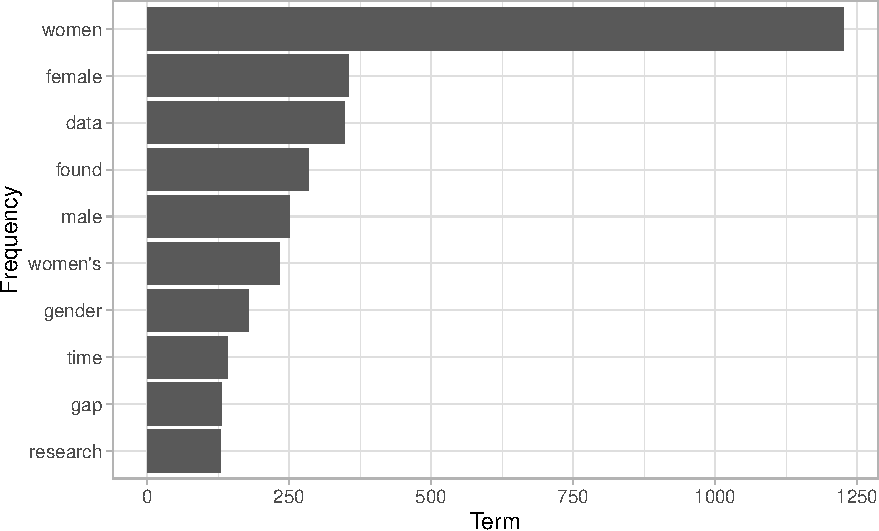
\includegraphics[width=0.7\linewidth]{report_files/figure-latex/TF-IDF plot-1} \end{center}

\hypertarget{term-frequency-tf}{%
\subsection{Term-Frequency (TF)}\label{term-frequency-tf}}

To deep dive into these frequencies, we then display a Term-Frequency
(TF) table providing information on term frequencies, their rank and
document frequencies. Indeed, the \emph{feature} lists the lemmatized
tokens, the \emph{frequency} provides the number of times the term is
found in the corpus (i.e.~global frequency), the \emph{rank} sorts the
terms by decreasing frequencies (i.e.~rank is inversely proportional to
the frequency), the \emph{docfreq} indicates the number of documents in
which the token is found (i.e.~document frequency).

The table below shows that \emph{woman} appears 1594 times in the corpus
and in all 16 documents (docfreq = 16) which means that it is not a
document-specific term. Moreover, it appears four times more than the
second most frequent term \emph{female}.

\begin{table}

\caption{\label{tab:term frequency}Term frequencies}
\centering
\begin{tabular}[t]{c|c|c|c}
\hline
feature & frequency & rank & docfreq\\
\hline
woman & 1594 & 1 & 16\\
\hline
female & 395 & 2 & 15\\
\hline
datum & 358 & 3 & 16\\
\hline
male & 334 & 4 & 16\\
\hline
find & 298 & 5 & 16\\
\hline
time & 260 & 6 & 16\\
\hline
gender & 256 & 7 & 16\\
\hline
study & 224 & 8 & 15\\
\hline
gap & 176 & 9 & 16\\
\hline
sex & 172 & 10 & 15\\
\hline
\end{tabular}
\end{table}

\hypertarget{term-frequency-versus-document-frequency}{%
\subsection{Term-Frequency versus
Document-Frequency}\label{term-frequency-versus-document-frequency}}

The below graph gives an overall graphical view of the previous table
indicating 1) the term-frequency and 2) whether a word is specific to a
document or not (i.e.~document-frequency). As observed previously, we
see that \emph{woman} is the most frequent term in the corpus and that
it is not document-specific since it is the most frequent term over all
chapters of the book. On the contrary, the terms \emph{trial} and
\emph{tax} are less frequent overall and also less frequent in documents
meaning that they are more specific to some chapters (i.e.~documents) of
the book.

Since we observe that \emph{woman} has a very large term-frequency and
is not document-specific, we decide to remove this term for the rest of
our analysis because we believe it will hide some important and
interesting insights as it will always appear as the top frequency in
all documents.

{[}Can we use a nicer looking theme ?{]}

\begin{center}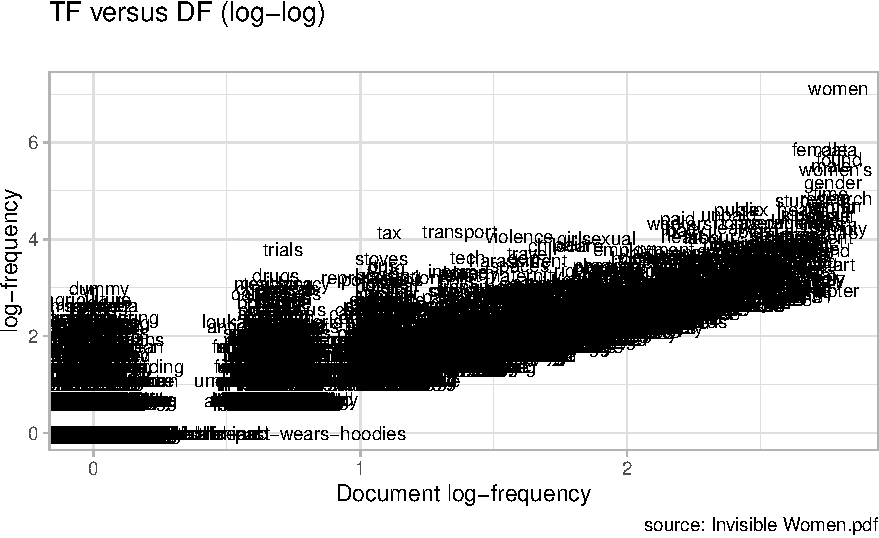
\includegraphics[width=0.7\linewidth]{report_files/figure-latex/TF vs DF-1} \end{center}

\hypertarget{term-frequency-by-document}{%
\subsection{Term-Frequency by
Document}\label{term-frequency-by-document}}

The plot below shows the ten most frequent terms for chapters of the
book {[}how are the chapters chosen?{]}. It would have been interesting
to have the top frequencies of each document but there would have been
an information overload as there are 16 chapters so we decided not to
display it.

{[}I dont understand how these ten most frequent terms are chosen ? they
are not the ten overall msot frequent ! it's confusing because they dont
match the order of the ten msot frequent terms overall !!!{]}

First, we see that Chapter 10 (i.e.~text10), namely \textbf{The Drugs
Don't Work}, is associated with \emph{sex}, \emph{drug} and
\emph{study}. In the previous plot (TF versus DF), we saw that
\emph{sex} and \emph{study} are not document-specific but that
\emph{drug} is more document-specific. Therefore, we can assume that
\emph{drug} is more specific to chapter 10 then the two other terms.
Nevertheless, we do not want to jump to conclusion right now and the
document-specificity of terms will be explored deeper later. Second,
chapter 13, \emph{From Purse to Wallet} seems to only be associated to
\emph{tax} and as well as \emph{drug}, \emph{tax} is more
document-specific. Third, chapter 14, \emph{Women's Rights are Human
Rights} is only associated to \emph{female}. Fourth, chapter 3,
\emph{The Long Friday} is related to \emph{pay}, \emph{leave} and
\emph{time} and lastly, chapter 4, \emph{Myth of Meritocracy} is equally
associated to \emph{female} and \emph{male}.

Even though some of those words are informative, others are much less
insightful. Indeed, it is not enlightening to have \emph{female}
associated to one document as the whole book is about feminism.

\begin{center}\includegraphics[width=0.7\linewidth]{report_files/figure-latex/term-frequency by document plot-1} \end{center}

\hypertarget{zipfs-law}{%
\subsection{Zipf's Law}\label{zipfs-law}}

The Zipf's law shows the distribution of words used in a corpus by
plotting the term-frequencies against their ranks and, it says that the
frequency of a token is inversely proportional to its rank. Therefore,
the below plot (on a log-log scale) shows a negative linear relation
(the original distribution (non log-log) is a negative exponential
function).

This plot shows that \emph{female}, \emph{datum}, \emph{male},
\emph{find} and \emph{time} are the most frequent terms of the corpus
probably indicating that they are not chapter-specific but frequent in
all chapters of the book. Indeed, although the Zipf's Law do not provide
precise information on document specificity, there is a very low
probability that these terms are specific to one or few chapters that
are sufficiently lengthy to make them appear as much. Therefore,
according to the Zipf's law, these terms are very frequent in the
overall corpus and consequently could hide some meaningful information
as they are not considered stop words {[}can we explain this a bit
better?{]}. The Zipf's law now leads us to move to look at weighted
frequencies.

\begin{verbatim}
#> Warning: Removed 5 rows containing missing values (geom_label).
\end{verbatim}

\begin{center}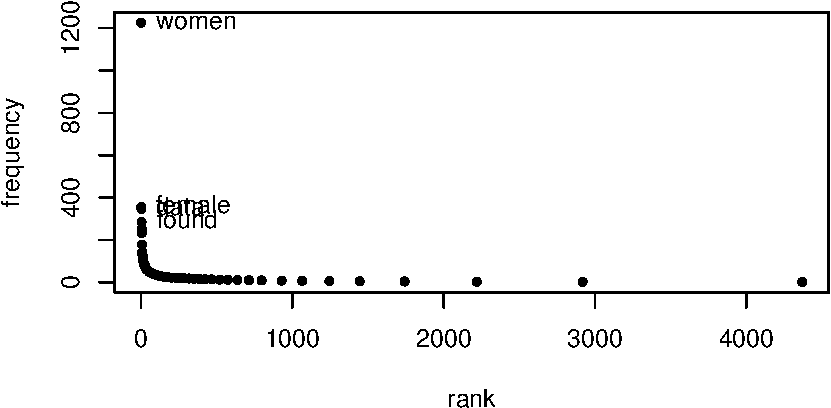
\includegraphics[width=0.7\linewidth]{report_files/figure-latex/Zipf law plot-1} \end{center}

\hypertarget{term-frequency-and-inverse-document-matrix-tf-idf}{%
\subsection{Term-Frequency and Inverse-Document Matrix
(TF-IDF)}\label{term-frequency-and-inverse-document-matrix-tf-idf}}

The TF-IDF matrix is a weighted document-feature matrix displaying term
frequency--inverse document frequency that shows how important a word is
to a document. In other words, it is used to re-balance a term frequency
with respect to its document-specificity.

The below output is the document-feature matrix of 16 documents and
5'741 features which shows the weighted frequencies of each token by
chapters of the book. The sparsity (83.77\%) increases a bit {[}add the
amount of the increase{]} compared to the DTM matrix when \emph{women}
is not removed. {[}explain why it induces an increase in sparsity{]}

\begin{verbatim}
#> Document-feature matrix of: 16 documents, 5,741 features (83.77% sparse) and 0 docvars.
#>        features
#> docs    sexist  joke town karlskoga sweden   hit initiative  lens
#>   text1  0.718 0.903 5.42      6.02   1.08 0.204      0.505 0.903
#>   text2  0     0     0         0      1.44 0.204      0     0    
#>   text3  0     0     0         0      2.51 0.612      0     0    
#>   text4  1.436 0     0         0      0    0          0.505 0    
#>   text5  0     0     0         0      0    0          0     0    
#>   text6  0.359 0     0         0      0    0.204      0     0    
#>        features
#> docs    harsh glare
#>   text1 0.903 0.903
#>   text2 0     0    
#>   text3 0     0    
#>   text4 0.903 0    
#>   text5 0     0    
#>   text6 0     0    
#> [ reached max_ndoc ... 10 more documents, reached max_nfeat ... 5,731 more features ]
\end{verbatim}

The following plot shows the twenty largest TF-IDF and their respective
terms. Note that it is equal to the result of computing for each term
the maximum TF-IDF over all chapters of the book. The output shows that
\emph{tax} has the largest TF-IDF (i.e.~has the largest weighted
frequency) in at least one chapter of the book and that \emph{trial},
\emph{drug} and \emph{dummy} appear also quite often in the corpus and
in few documents.

\begin{center}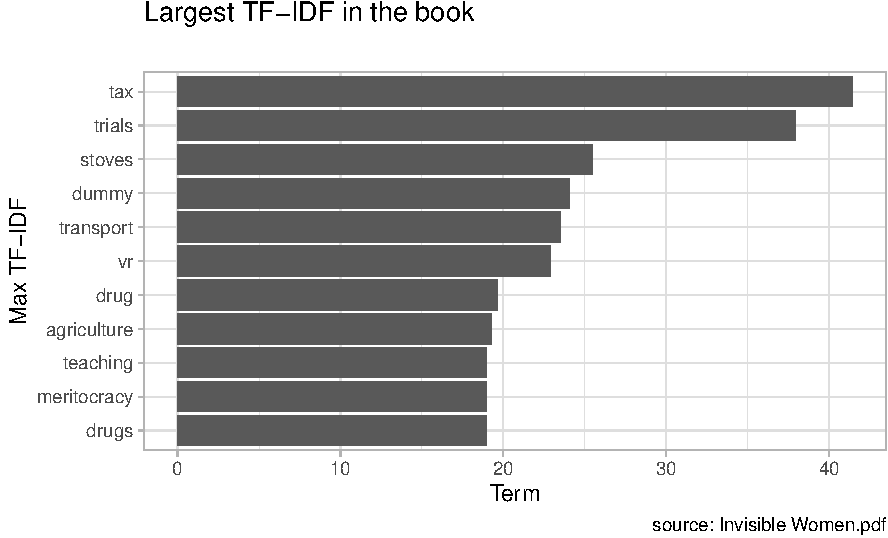
\includegraphics[width=0.7\linewidth]{report_files/figure-latex/max tf-idf-1} \end{center}

\hypertarget{tf-idf-by-document}{%
\subsection{TF-IDF by Document}\label{tf-idf-by-document}}

After looking at the overall largest TF-IDFs in the corpus, we look at
the ten largest TF-IDFs by chapters of the book. The following plot
shows that chapter 10, \emph{The Drugs Don't Work}, is now associated
with \emph{trial} and \emph{drug}, that \emph{tax} is really frequent in
chapter 13 \emph{From Purse to Wallet} so we can now state that it is
specific to this chapter and that chapter 14, \emph{Women's Rights are
Human Rights}, is in fact more specifically associated with the term
\emph{interrupt} than with the term \emph{female} as shown in the
\emph{Term-Frequency by Document} section of the \textbf{Exploratory
Data Analysis (EDA)}.

{[}what's the firm term ? vr ? {]}

\begin{center}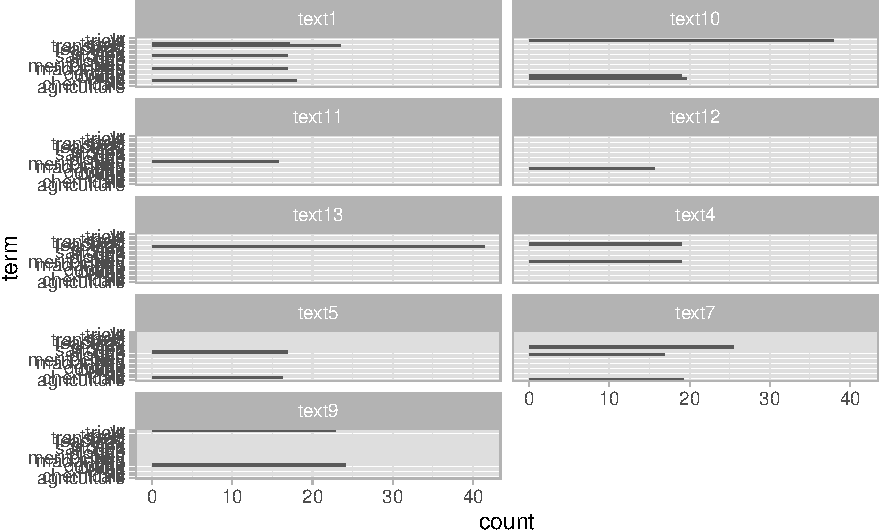
\includegraphics[width=0.7\linewidth]{report_files/figure-latex/tfidf by document plot-1} \end{center}

\hypertarget{keyness}{%
\subsection{Keyness}\label{keyness}}

The keyness measure is a chi-square test of independence indicating
whether some terms are characteristic of a target compared to a
reference. We illustrate the keyness by investigating why the vague term
\emph{interrupt} is associated to chapter 14 \emph{Women's Rights are
Human Rights}. Thus, we compute its keyness and compare it to the other
chapters (i.e.~reference).

The plot below allows us to see that this chapter is characterized by
the terms \emph{party}, \emph{politician}, \emph{election} or even
\emph{candidate} and to conclude at first glance that this chapter is
more about political topics than the rest of the corpus.

\begin{center}\includegraphics[width=0.7\linewidth]{report_files/figure-latex/keyness-1} \end{center}

Then, we compute for each chapter of the book the keyness of terms in
order to better understand what each chapter is about. The following
visualization is an animated illustration (in a gif format). Each
chapter is then at some point the target and the reference.

Chapter 1 \emph{Can Snow-Clearing be Sexist?} displays terms related to
public transportation and cities' infrastructure, chapter 2 \emph{Gender
Neutral With Urinals} mentions terms in connection with public spaces
and dangerous behaviors, chapter 3 \emph{The Long Friday} seem to be
about parental benefits in the workplace, chapter 4 \emph{The Myth of
Meritocracy} elaborates on success, chapter 5 \emph{The Henry Higgins
Effect} is a bit more difficult to grasp but uses terms related to
chemicals and effect on health such as cancer, chapter 6 \emph{Being
Worth Less Than a Shoe} is also less specific to one vocabulary type but
seems to be about profession and precariousness, chapter 7 \emph{The
Plough Hypothesis} uses terms related to agriculture, chapter 8
\emph{One-Size-Fits-Men} seems to be about technologies like smartphones
and data science, chapter 9 \emph{A Sea of Dudes} uses vocabulary
connected to automobiles, chapter 10 \emph{The Drugs Don't Work} is
about clinical trials, chapter 11 \emph{Yentl Syndrome} uses a medical
vocabulary, chapter 12 \emph{A Costless Resource to Exploit} seems to be
about economics, chapter 13 \emph{From Purse to Wallet} is connected to
household consumption, chapter 14 \emph{Women's Rights are Human Rights}
is about politics, chapter 15 \emph{Who Will Rebuild?} implies a topic
surrounding rebuilding a more peaceful world and chapter 16 \emph{It's
Not the Disaster that Kills You} evolves around extreme poverty in the
world.

\begin{center}\animategraphics[width=0.7\linewidth,controls,loop]{0.0666666666666667}{report_files/figure-latex/keyness2-}{1}{16}\end{center}

\hypertarget{link-between-words}{%
\subsection{Link between words}\label{link-between-words}}

Here, we look at how words co-occur and how inter-connected they are and
to do so, we first compute the co-occurrences between terms.

The feature co-occurrence matrix is a 5,741 by 5,741 matrix (32,959,081
elements) in which is displayed the number of times two terms co-occur
(i.e.~co-occurrence frequency) in the corpus. Because of the large size
of the matrix, we decide to reduce its size by keeping only
co-occurrences greater than 110. The latter condition allows us to focus
our attention on terms that appear the most together in the corpus,
implying that they have a specific connection of interest in the context
of the book. After applying this condition to the matrix, we get the
following smaller feature co-occurrence matrix of dimensions 20 by 20
features (400 elements).

\begin{verbatim}
#> Feature co-occurrence matrix of: 20 by 20 features.
#>         features
#> features datum male find time gender study  gap  sex  pay report
#>   datum   4481 8548 6860 5544   5961  5258 4026 4303 3080   3346
#>   male    8548 4854 7730 5167   6103  6348 3859 5317 2285   2995
#>   find    6860 7730 3485 5218   4917  6060 3362 5104 3017   2810
#>   time    5544 5167 5218 3000   4469  3644 3291 2252 5227   2250
#>   gender  5961 6103 4917 4469   2529  3490 2884 2746 3065   2414
#>   study   5258 6348 6060 3644   3490  2622 2456 5277 1636   2181
#>   gap     4026 3859 3362 3291   2884  2456 1008 1864 2461   1410
#>   sex     4303 5317 5104 2252   2746  5277 1864 3943  562   1794
#>   pay     3080 2285 3017 5227   3065  1636 2461  562 2878   1144
#>   report  3346 2995 2810 2250   2414  2181 1410 1794 1144    876
#> [ reached max_feat ... 10 more features, reached max_nfeat ... 10 more features ]
\end{verbatim}

Using the above feature co-occurrences matrix, we generate a network
(object) displaying visually the inter-connections of interest between
the co-occurring terms appearing more than 110 times in the corpus. To
generate a readable network of co-occurrences, we add a second condition
on the co-occurring features and we keep only the co-occurrences greater
than 2,100.

The below network reveals that the terms \emph{datum}, \emph{male} and
\emph{find} are central and co-occur a lot with the surrounding terms.
The output shows a surprising finding which is that for a book named
\textbf{Invisible Women}, the term \emph{female} is not a central term
co-occurring the most with other terms. Therefore, to dig deeper into
this finding, we decide to re-introduce the term \emph{woman} and we
find an even more surprising result which is that \emph{woman} is still
not at the center of the co-occurrences despite its significantly large
frequency (1,594 out of 36,160 or 4.4\% of all frequencies).

\begin{center}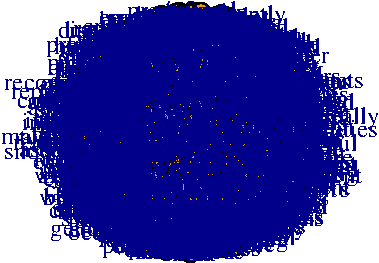
\includegraphics[width=0.7\linewidth]{report_files/figure-latex/network-1} \end{center}

\hypertarget{dispersion-plot}{%
\subsection{Dispersion Plot}\label{dispersion-plot}}

After investigating term co-occurrences, we look at how terms move
together in the book. Dispersion or X-Ray plots inspect where a specific
token is used in each text by locating a pattern in each text.

The below lexical dispersion plot shows how the terms \emph{female} and
\emph{male} move along the chapters. First, \emph{male} is found in all
chapters but only once in chapter 6 \emph{Being Worth Less Than A Shoe}
whereas as \emph{female} is only not found in chapter 15, namely
\emph{Who Will Rebuild}. When considering the implication of the title
of this chapter, this finding seems a bit curious. Second, these two
terms often seem to appear together at some point in chapters. Third, we
also see that they are both present in chapters 4 \emph{The Long Friday}
and 14 \emph{Women's Rights are Human Rights} at a higher frequency but
not necessarily used at the same location suggesting that the author
might compare the two more in these chapters.

\begin{center}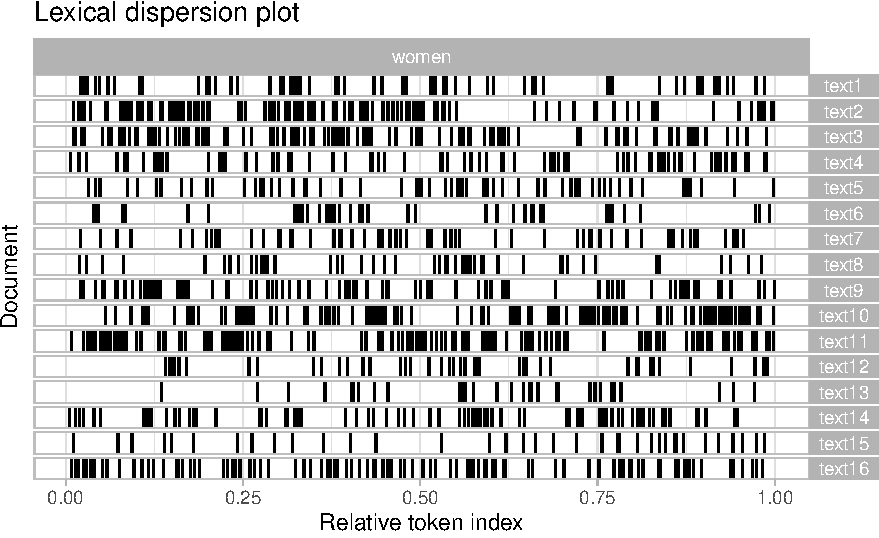
\includegraphics[width=0.7\linewidth]{report_files/figure-latex/xray plot-1} \end{center}

After exploring the movements of \emph{female} and \emph{male}, we look
at the movements between \emph{female} and \emph{sex}. Note that here
\emph{sex} is reduced to its lemma so it could refer to the gender, the
nature of a relation or any other terms related to sexuality. The below
plot shows that the term \emph{sex} is more specific to chapter 10
\emph{The Drugs Don't Work} and that \emph{female} and \emph{sex} are
not necessarily associated.

\begin{center}\includegraphics[width=0.7\linewidth]{report_files/figure-latex/xray-plot 2 patterns-1} \end{center}

Lastly, we explore the movements of \emph{male} and \emph{sex}. This
following plot reveals that \emph{male} and \emph{sex} seem to be used
together most often in Chapter 10 \emph{The Drugs Don't Work}.
Furthermore, using previous results where we find that chapter 10 is
associated with \emph{trial} and \emph{drug}, we can conclude that this
chapter probably focuses on clinical trials and gender.

\begin{center}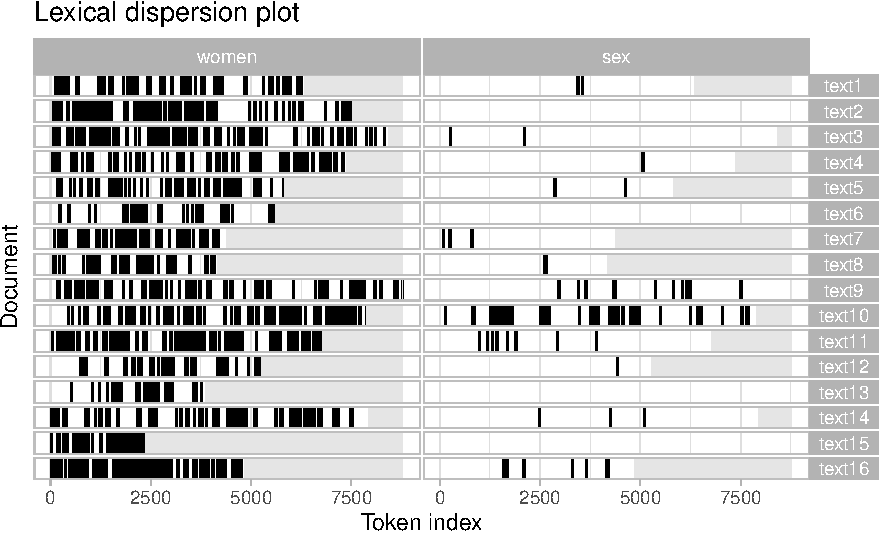
\includegraphics[width=0.7\linewidth]{report_files/figure-latex/xray plot 2 patterns-1} \end{center}

\hypertarget{lexical-diversity}{%
\subsection{Lexical Diversity}\label{lexical-diversity}}

Lexical diversity is a diversity index that measures the richness of the
vocabulary in one document.

\hypertarget{token-type-ratio-ttr}{%
\subsubsection{Token-Type Ratio (TTR)}\label{token-type-ratio-ttr}}

The TTR is a diversity measure indicating a document's richness in the
number of token types. The more types of tokens are found in a document,
the richest is the vocabulary of this specific document. The closest to
1 the TTR is, the richest the vocabulary of a document is. We need to be
careful with the TTR measure because it is dependent on the length of
the document. TTR is computed using the document-term matrix.

The below graph sorts chapters of the book by descending TTR. According
to TTR, chapter 15 \emph{Who Will Rebuild?} has the richest vocabulary
among all chapters of the book with a TTR of 0.592 and chapter 3
\emph{The Long Friday} has the poorest with a TTR of 0.374. Overall, the
richness of vocabulary is not very diverse which could be explained by
the fact that the author focuses on the specific gender issue, therefore
using repetitively gender-specific terms.

\begin{center}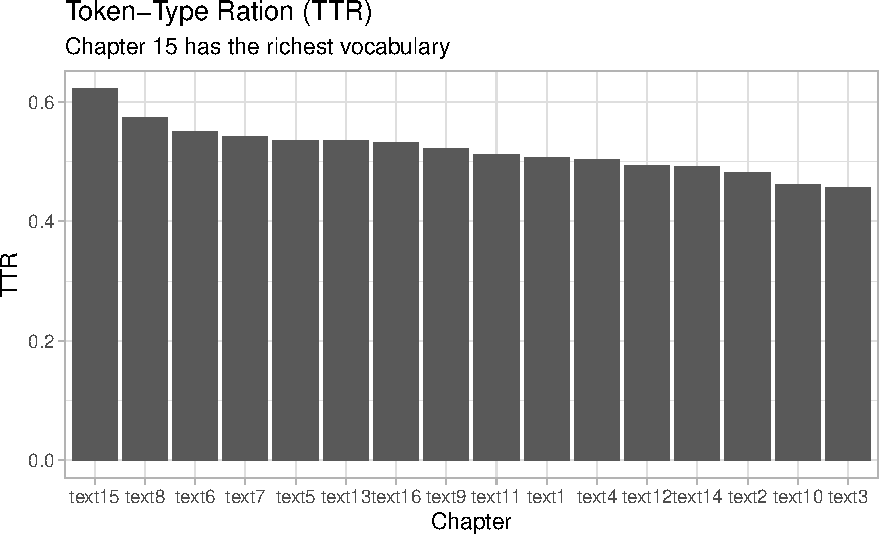
\includegraphics[width=0.7\linewidth]{report_files/figure-latex/TTR plot-1} \end{center}

\hypertarget{moving-average-token-type-ratio-mattr}{%
\subsubsection{Moving-Average Token-Type Ratio
(MATTR)}\label{moving-average-token-type-ratio-mattr}}

The Moving-Average Token-Type Ratio is an average of the Token-Type
Ratio. It is an algorithm using windows of the text to compute the TTR
and repeating several times over different windows of the same size the
TTR computation. The advantage of the MATTR is that it is less dependent
on the length of the document than the TTR. Note that a too large window
can produce an error since no local TTR can be computed and a too small
window results in pointless values (always 1). MATTR is computed using
ordered tokens.

The below graph shows the the Moving-Average Token-Type Ratio and shows
that the MATTR among chapters are very similar and that it ranges from
0.725 to 0.798 over all chapters of the book. According to the MATTR,
chapter 15 \emph{Who Will Rebuild?} still has the richest vocabulary
with an MATTR of 0.798.

\begin{center}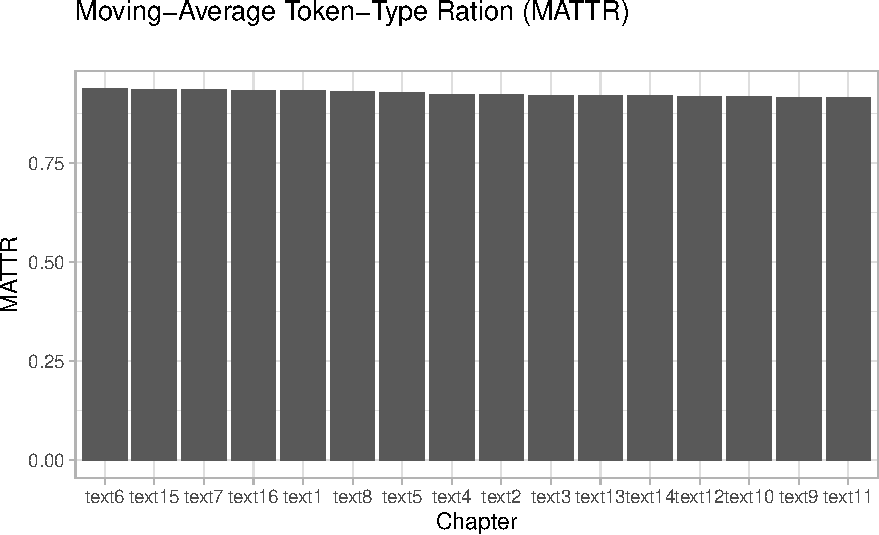
\includegraphics[width=0.7\linewidth]{report_files/figure-latex/MATTR plot-1} \end{center}

\hypertarget{analysis}{%
\section{4. Analysis}\label{analysis}}

This section dives deeper into the analysis of the content of the
corpus. Each part of our analysis is supported by well-designed relevant
charts and graphs using the \textbf{ggplot2}, \textbf{sentimentr},
\textbf{reshape2}, \textbf{quanteda.textmodels}, \textbf{seededlda} and
\textbf{text2vec} packages {[}VERIFY IF ALL THESE PACKAGES PROVIDE OR
HELP PROVIDE A GRAPHICAL REPRESENTATION{]}.

-\textgreater{} talk about the complexity of the book: specify the
length of the text before and after the cleaning ? assess the difference
(big or small) and interpret (if big, most words are bringing no
information, if small, most terms are insightful) ? {[}DO YOU HAVE ANY
OTHER IDEAS THAT COULD ASSESS THE COMPLEXITY OF THE TEXT ?{]}

-\textgreater{} talk about the uniqueness of the data : {[}NOT SURE WHAT
TO MENTION HERE BUT MUST BE MENTIONNED{]}

\hypertarget{sentiment-analysis}{%
\subsection{Sentiment Analysis}\label{sentiment-analysis}}

Now that the content of the corpus is cleaned and that we have explored
its content, we proceed to its sentiment analysis (i.e.~opinion mining)
which qualifies or quantifies the sentiment emerging from one text
(i.e.~chapter). To proceed to the sentiment analysis, we use two
approaches. The first one uses qualifiers (i.e.~dictionary-based) and
the second one uses values (i.e.~value-based).

When analyzing the sentiment emerging from a document, we do not use the
data in which stop words are removed since they might be in the
sentiment dictionary and provide useful insight.

\hypertarget{dictionary-based}{%
\subsubsection{Dictionary-Based}\label{dictionary-based}}

The dictionary-based sentiment analysis matches tokens from each
document to a reference dictionary with token values and then, look for
word polarity. The sentiment is the average over token values of the
document.

The disadvantage of the dictionary-based sentiment analysis is that the
negative forms are not taken into consideration. For example, in the
sentence \emph{I don't enjoy the show}, the sentence will be considered
positive because it will not consider the contraction \emph{don't} but
only the word \emph{enjoy}.

The following non-exhaustive table shows the number of terms matched
with a \textbf{positive}, \textbf{negative}, \textbf{neg\_positive} or
\textbf{neg\_negative} sentiment for each document (i.e.~chapter). For
example, in chapter one, 142 terms are matched with a negative sentiment
and 167 are found matched with a positive sentiment.

\begin{table}

\caption{\label{tab:dictionary-based analysis}Sentiment Analysis (Dictionary-Based)}
\centering
\begin{tabular}[t]{l|r|r}
\hline
document & negative & positive\\
\hline
text1 & 142 & 167\\
\hline
text2 & 408 & 177\\
\hline
text3 & 176 & 241\\
\hline
text4 & 254 & 300\\
\hline
text5 & 227 & 129\\
\hline
text6 & 232 & 123\\
\hline
text7 & 128 & 150\\
\hline
text8 & 130 & 127\\
\hline
text9 & 288 & 252\\
\hline
text10 & 330 & 153\\
\hline
text11 & 345 & 132\\
\hline
text12 & 112 & 168\\
\hline
text13 & 118 & 107\\
\hline
text14 & 299 & 218\\
\hline
text15 & 86 & 97\\
\hline
text16 & 321 & 120\\
\hline
\end{tabular}
\end{table}

The below graph is a representation of the previous table. For each
chapter of the book, we see the proportion of terms matched with a
positive, negative, negative positive or negative negative sentiment.

Overall, positive and negative sentiments are found in all 16 chapters
of the book. Although, more terms are recognized as negative (3,596)
than as positive (2,661) indicating that the frequency of negative terms
is higher than the one of positive terms.

\begin{center}\includegraphics[width=0.7\linewidth]{report_files/figure-latex/dictionary-based analysis plot2-1} \end{center}

\hypertarget{valence-shifters}{%
\subsubsection{Valence Shifters}\label{valence-shifters}}

The valence shifters approach uses positive/negative sentiment scores
(i.e.~value-based) to extract the sentiment of a document. Here, we use
two dictionaries, a polarized words dictionary where we find a list of
terms communicating a positive or negative attitude and a
valence-shifters dictionary which provides terms that alter or intensify
the meaning of the polarized words.

The next table shows the first ten words of the polarized words
dictionary and their numerical score.

\begin{table}

\caption{\label{tab:polarized words dictionary}Polarized Words Dictionary}
\centering
\begin{tabular}[t]{l|r}
\hline
x & y\\
\hline
a plus & 1.00\\
\hline
abandon & -0.75\\
\hline
abandoned & -0.50\\
\hline
abandoner & -0.25\\
\hline
abandonment & -0.25\\
\hline
abandons & -1.00\\
\hline
abducted & -1.00\\
\hline
abduction & -0.50\\
\hline
abductions & -1.00\\
\hline
aberrant & -0.60\\
\hline
\end{tabular}
\end{table}

The next table shows the first ten words of the valence-shifters
dictionary and their numerical score.

\begin{table}

\caption{\label{tab:valence-shifters dictionary}Valence-Shifters Dictionary}
\centering
\begin{tabular}[t]{l|l}
\hline
x & y\\
\hline
absolutely & 2\\
\hline
acute & 2\\
\hline
acutely & 2\\
\hline
ain't & 1\\
\hline
aint & 1\\
\hline
almost & 3\\
\hline
although & 4\\
\hline
aren't & 1\\
\hline
arent & 1\\
\hline
barely & 3\\
\hline
\end{tabular}
\end{table}

To proceed to the valance-shifters sentiment analysis, we extract the
sentences from the text and we compute the sentiment value for each
sentence. Because the column \emph{word\_count} had NAs, we remove rows
that have no available information since no sentiment can be extracted.
Moreover, we do not assign weights to certain types of sentences
(e.g.~questions) since we believe that the sentence type does not have a
particular influence in our analysis.

The below output displays the sentiment value of the first ten sentences
of the corpus and indicates the number of terms for each. Anything below
-0.05 is considered negative and anything above 0.05 is considered
positive. Anything in between is considered neutral. For example, the
first sentence is negative (-0.408), the seventh sentence is neutral (0)
and the eigth sentence is positive (0.332).

\begin{table}

\caption{\label{tab:sentiment analysis}Sentiment Values by Sentence}
\centering
\begin{tabular}[t]{r|r|r|r}
\hline
element\_id & sentence\_id & word\_count & sentiment\\
\hline
1 & 1 & 6 & -0.408\\
\hline
1 & 2 & 6 & 0.245\\
\hline
1 & 3 & 33 & 0.096\\
\hline
1 & 4 & 33 & -0.296\\
\hline
1 & 5 & 14 & -0.535\\
\hline
1 & 6 & 26 & 0.078\\
\hline
1 & 7 & 14 & 0.000\\
\hline
1 & 8 & 54 & 0.332\\
\hline
1 & 9 & 55 & 0.146\\
\hline
1 & 10 & 20 & 0.145\\
\hline
\end{tabular}
\end{table}

After taking a look at the sentiment score for each sentence, we zoom
out to look into the sentiment score by chapter of the book. The
\emph{ave\_sentiment} column gives the average sentiment (i.e) score by
chapter.

The below table displays the average sentiment scores by chapter in a
decreasing fashion. According to the table, chapter 4 \emph{The Myth of
Meritocracy} has the greatest positive average. In total, five chapters
have a positive sentiment (i.e.~scores above 0.05), four have a negative
sentiment (i.e.~scores below -0.05) and seven chapters have a neutral
sentiment (i.e.~scores between -0.05 and 0.05). -\textgreater{} CORRECT
ONCE PROBLEM FIXED

{[}PROBLEM IL NY A PAS TOUS LES CHAPITRES ET LES CHAPITRES APPARAIISSENT
PLUSIEURS FOIS{]}

\begin{table}

\caption{\label{tab:sentiment analysis by document}Sentiment Values by Chapter}
\centering
\begin{tabular}[t]{l|r|r|r}
\hline
document & word\_count & sd & ave\_sentiment\\
\hline
chapter 4 & 6520 & 0.323 & 0.118\\
\hline
chapter 7 & 3858 & 0.262 & 0.108\\
\hline
chapter 1 & 5598 & 0.262 & 0.080\\
\hline
chapter 12 & 4496 & 0.272 & 0.061\\
\hline
chapter 3 & 7476 & 0.255 & 0.057\\
\hline
chapter 8 & 3683 & 0.247 & 0.048\\
\hline
chapter 13 & 3389 & 0.242 & 0.038\\
\hline
chapter 15 & 2066 & 0.313 & 0.018\\
\hline
chapter 5 & 5167 & 0.253 & -0.001\\
\hline
chapter 9 & 7737 & 0.280 & -0.002\\
\hline
chapter 14 & 6963 & 0.289 & -0.007\\
\hline
chapter 10 & 6900 & 0.278 & -0.040\\
\hline
chapter 6 & 4908 & 0.266 & -0.057\\
\hline
chapter 11 & 6023 & 0.360 & -0.104\\
\hline
chapter 2 & 6617 & 0.335 & -0.105\\
\hline
chapter 16 & 4232 & 0.366 & -0.204\\
\hline
\end{tabular}
\end{table}

Sentiment changes as sentences change. Thus, in order to better track
the evolution of the sentiment, we plot the sentiment scores' evolution
by chapter of the book (i.e.~by document).

The below plot shows the range of sentiment scores by chapter indicating
how much sentiment evolves throughout the sentences.

PROBLEM NOT ALL CHAPTERS ARE ON THE PLOT

\begin{center}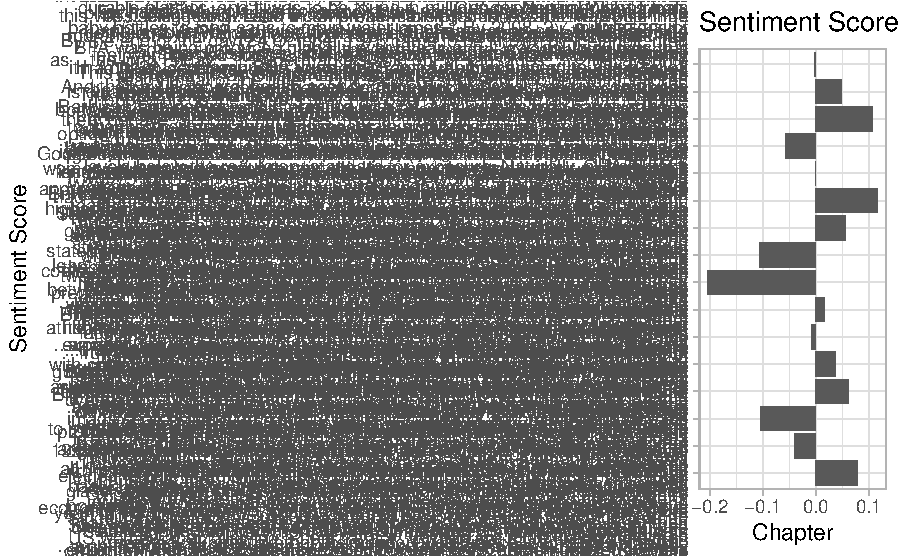
\includegraphics[width=0.7\linewidth]{report_files/figure-latex/sentiment analysis by document plot-1} \end{center}

\hypertarget{similarities-and-clustering}{%
\subsection{Similarities and
Clustering}\label{similarities-and-clustering}}

Similarity is a proximity measure. Once can measure similarity between
terms to see if they are used in the same context or similarity between
documents and see whether a document uses the same tokens.

\hypertarget{similarities-between-documents}{%
\subsubsection{Similarities between
Documents}\label{similarities-between-documents}}

\hypertarget{jaccard-index}{%
\paragraph{Jaccard Index}\label{jaccard-index}}

To study similarities between chapters (i.e.~documents) of the book, we
first compute the Jaccard index matrix displaying the relative number of
common words using the TF-IDF matrix.

\begin{center}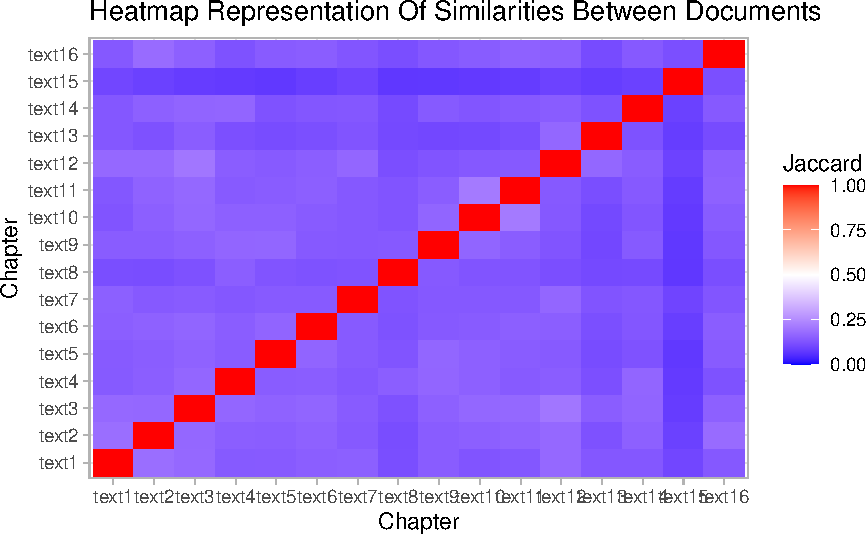
\includegraphics[width=0.7\linewidth]{report_files/figure-latex/Jaccard-1} \end{center}

\hypertarget{cosine}{%
\paragraph{Cosine}\label{cosine}}

Then, we compute the cosine similarity matrix.

\begin{center}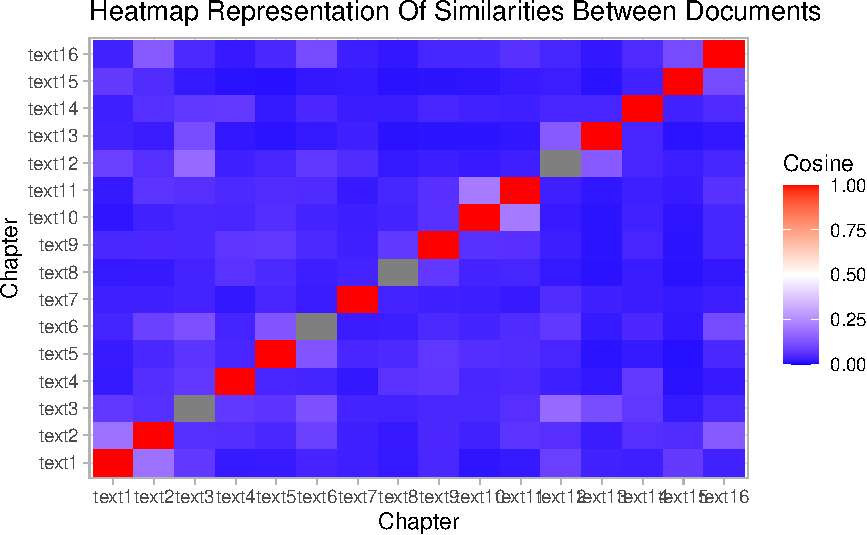
\includegraphics[width=0.7\linewidth]{report_files/figure-latex/Cosine-1} \end{center}

\hypertarget{euclidean-similarity}{%
\paragraph{Euclidean similarity}\label{euclidean-similarity}}

Finally, we compute the Euclidean-based similarity matrix. Is there a
clearer separation between documents ? compare with above heatmaps !
Which documents are similar ? Are their groups ?

\begin{center}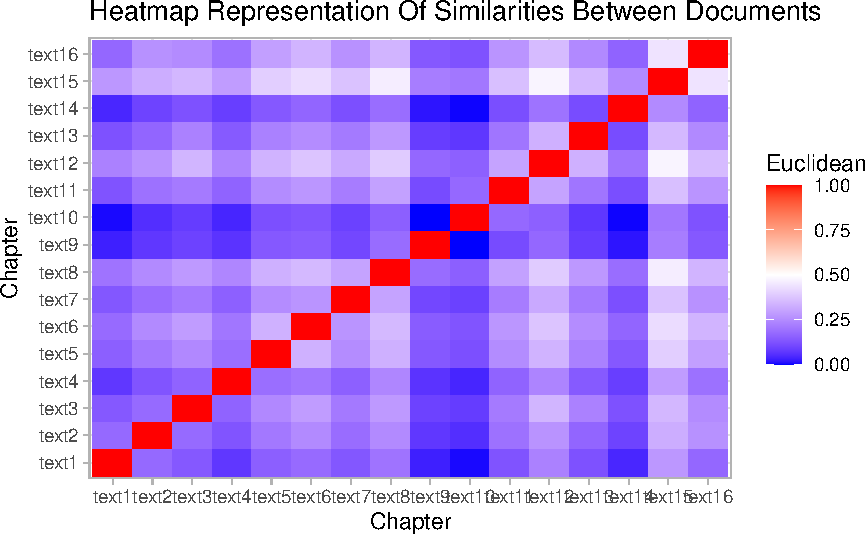
\includegraphics[width=0.7\linewidth]{report_files/figure-latex/Euclidean-1} \end{center}

\hypertarget{clustering-of-documents}{%
\subsubsection{Clustering of Documents}\label{clustering-of-documents}}

To proceed to clustering documents, we need to build the dissimilarities
and/or vector space model (VSM) on which we can apply the clustering
methods. There are two approaches to clustering. One is based on
distances (i.e.~hierarchical clustering) and the other one is based on
features co-occurrences? (i.e.~partitioning).

Clusters are difficult to interpret. This is why we can look at the most
frequent terms in each cluster to understand better what they are
grouping.

\hypertarget{hierarchical-clustering}{%
\paragraph{Hierarchical Clustering}\label{hierarchical-clustering}}

Hierarchical clustering is based on distances and applied on the
dissimilarities.

\hypertarget{inverted-jaccard-dissimilarity-matrix}{%
\subparagraph{Inverted Jaccard Dissimilarity
Matrix}\label{inverted-jaccard-dissimilarity-matrix}}

The inverted Jaccard dissimilarity matrix seems to show that there are
two clusters. One grouping chapter 15 \emph{Who Will Rebuild} and the
other one grouping the rest of the book.

\begin{center}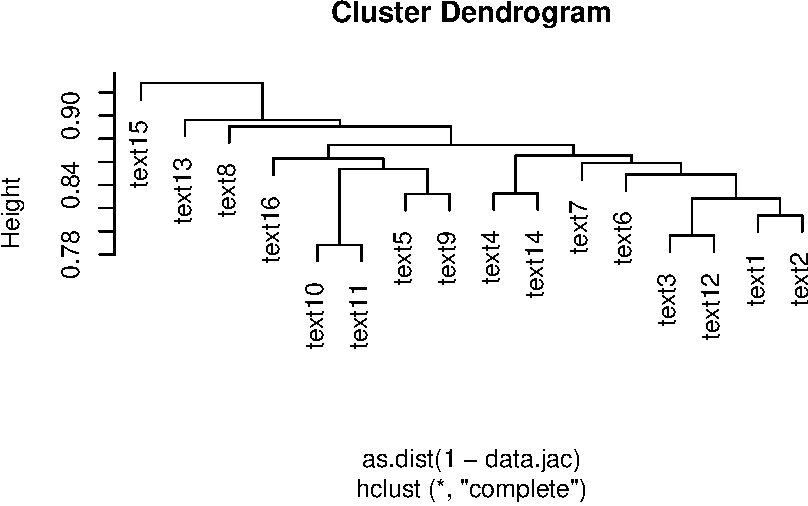
\includegraphics[width=0.7\linewidth]{report_files/figure-latex/Jaccard inverted-1} \end{center}

From the clustering, we extract the ten words that are the most used.

\begin{verbatim}
#>  text1  text2  text3  text4  text5  text6  text7  text8  text9 
#>      1      1      1      2      2      2      1      3      2 
#> text10 text11 text12 text13 text14 text15 text16 
#>      2      2      1      4      1      5      6
\end{verbatim}

\begin{table}

\caption{\label{tab:Jaccard cutree}Ten Most Frequent Terms By Cluster}
\centering
\begin{tabular}[t]{l|l|l|l|l|l}
\hline
Clust.1 & Clust.2 & Clust.3 & Clust.4 & Clust.5 & Clust.6\\
\hline
transport & trial & keyboard & tax & rebuild & refugee\\
\hline
bus & drug & corpus & poverty & peace & violence\\
\hline
stove & dummy & voice & earner & orleans & shelter\\
\hline
interrupt & vr & pianist & marry & disaster & disaster\\
\hline
toilet & tech & algorithm & household & agreement & homeless\\
\hline
pedestrian & crash & recognition & file & miami & homelessness\\
\hline
travel & chemical & dataset & zombie & displace & conflict\\
\hline
party & pain & handspan & couple & fordham & ebola\\
\hline
plough & meritocracy & phone & income & gujarat & cyclone\\
\hline
agriculture & clinical & inch & youth & hurricane & camp\\
\hline
\end{tabular}
\end{table}

Using jaccard we still have two cluster that have terms the same
previous previous clustering using euclidean distance : transport and
medical, but the cluster 3 is different with top terms related to
disaster or war, rather than top terms related to cars.

\hypertarget{inverted-cosine-dissimilarity-matrix}{%
\subparagraph{Inverted Cosine Dissimilarity
Matrix}\label{inverted-cosine-dissimilarity-matrix}}

The inverted cosine dissimilarity matrix seems to show that there are
two clusters. One grouping chapters 4, 14, 5, 6, 10, 11 and 8, 9 and the
other one grouping chapters 1, 2, 15, 16, 7, 13, 3 and 12.

\begin{center}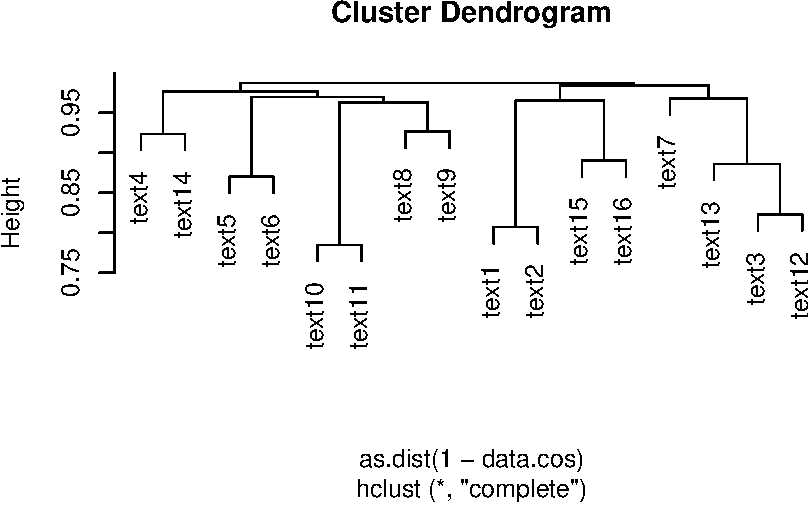
\includegraphics[width=0.7\linewidth]{report_files/figure-latex/cosine inverted-1} \end{center}

From the clustering, we extract the ten words that are the most used.

\begin{verbatim}
#>  text1  text2  text3  text4  text5  text6  text7  text8  text9 
#>      1      1      2      3      4      4      5      4      4 
#> text10 text11 text12 text13 text14 text15 text16 
#>      6      6      2      2      3      1      1
\end{verbatim}

\begin{table}

\caption{\label{tab:cosine cutree}Ten Most Frequent Terms By Cluster}
\centering
\begin{tabular}[t]{l|l|l|l|l|l}
\hline
Clust.1 & Clust.2 & Clust.3 & Clust.4 & Clust.5 & Clust.6\\
\hline
transport & tax & interrupt & dummy & stove & trial\\
\hline
bus & pay & candidate & vr & plough & drug\\
\hline
toilet & gdp & party & crash & agriculture & clinical\\
\hline
pedestrian & poverty & meritocracy & chemical & stave & pain\\
\hline
travel & childcare & politician & ppe & farmer & cell\\
\hline
violence & household & election & boler & agricultural & blood\\
\hline
disaster & marry & hire & worker & crop & fda\\
\hline
snow & offer & mp & stoffregen & farm & heart\\
\hline
sánchez & week & aw & tech & strength & disease\\
\hline
madariaga & carer & teach & keyboard & doss & medication\\
\hline
\end{tabular}
\end{table}

Here we have cluster top terms similar than using euclidean distance.

\hypertarget{euclidean-based-dissimilarity-matrix}{%
\subparagraph{Euclidean-based Dissimilarity
Matrix}\label{euclidean-based-dissimilarity-matrix}}

The Euclidean dissimilarity matrix seems to show that there are three
clusters. One grouping chapter 10 \emph{The Drugs Don't Work}, one
chapter 9 \emph{A Sea Of Dudes} and the other one the rest of the book.

\begin{center}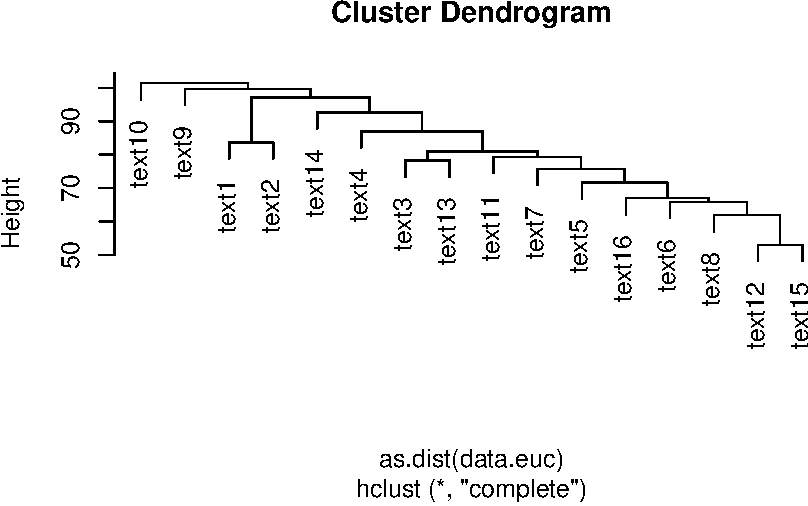
\includegraphics[width=0.7\linewidth]{report_files/figure-latex/Euclidean-based-1} \end{center}

From the clustering, we extract the ten words that are the most used.

\begin{verbatim}
#>  text1  text2  text3  text4  text5  text6  text7  text8  text9 
#>      1      2      2      2      2      2      2      2      3 
#> text10 text11 text12 text13 text14 text15 text16 
#>      4      2      2      5      6      2      2
\end{verbatim}

\begin{table}

\caption{\label{tab:Euclidean-based cutree}Ten Most Frequent Terms By Cluster}
\centering
\begin{tabular}[t]{l|l|l|l|l|l}
\hline
Clust.1 & Clust.2 & Clust.3 & Clust.4 & Clust.5 & Clust.6\\
\hline
pedestrian & toilet & dummy & trial & tax & interrupt\\
\hline
transport & stove & vr & drug & poverty & party\\
\hline
snow & violence & crash & cell & earner & candidate\\
\hline
sánchez & worker & boler & clinical & marry & politician\\
\hline
madariaga & pay & stoffregen & fda & household & election\\
\hline
travel & bus & tech & nih & file & mp\\
\hline
de & chemical & motion & blood & zombie & aw\\
\hline
trip & girl & seat & medication & couple & representation\\
\hline
favela & plough & belt & adr & income & political\\
\hline
clear & meritocracy & tin & animal & youth & ambition\\
\hline
\end{tabular}
\end{table}

It is interesting to observe that cluster one seems more to have words
about transport and work, cluster two about car, and cluster 3 about
medical.

\hypertarget{k-means}{%
\paragraph{K-Means}\label{k-means}}

K-means is applied on the features (i.e.~terms?) using TF-IDF.

\hypertarget{euclidean-based}{%
\subparagraph{Euclidean-Based}\label{euclidean-based}}

\begin{verbatim}
#>  text1  text2  text3  text4  text5  text6  text7  text8  text9 
#>      6      6      4      4      4      4      4      4      3 
#> text10 text11 text12 text13 text14 text15 text16 
#>      5      4      4      1      2      4      4
\end{verbatim}

\begin{table}

\caption{\label{tab:Euclidean-based km}Ten Most Frequent Terms By Cluster}
\centering
\begin{tabular}[t]{l|l|l|l|l|l}
\hline
Clust.1 & Clust.2 & Clust.3 & Clust.4 & Clust.5 & Clust.6\\
\hline
tax & interrupt & dummy & stove & trial & transport\\
\hline
poverty & party & vr & worker & drug & bus\\
\hline
earner & candidate & crash & violence & cell & toilet\\
\hline
marry & politician & boler & chemical & clinical & pedestrian\\
\hline
household & election & stoffregen & pay & fda & travel\\
\hline
file & mp & tech & plough & nih & snow\\
\hline
zombie & aw & motion & meritocracy & blood & sánchez\\
\hline
couple & representation & seat & disaster & medication & madariaga\\
\hline
income & political & belt & agriculture & adr & trip\\
\hline
youth & ambition & tin & pain & animal & de\\
\hline
\end{tabular}
\end{table}

Using kmean we have the cluster 2 that is different from other method,
with top terms related to politics.

\hypertarget{similarities-between-words}{%
\subsubsection{Similarities Between
Words}\label{similarities-between-words}}

Now we analyze similarities between words through chapters
(i.e.~documents). Because of the large number of words, we focus on word
frequency ranks smaller or equal to 40 (i.e.~40 most frequent words).

\hypertarget{cosine-1}{%
\paragraph{Cosine}\label{cosine-1}}

What words are similar ? It means they are used in similar proportion
through documents.

\begin{verbatim}
#>  [1] "woman"      "female"     "datum"      "male"       "find"      
#>  [6] "time"       "gender"     "study"      "gap"        "sex"       
#> [11] "pay"        "report"     "research"   "increase"   "country"   
#> [16] "don"        "world"      "result"     "leave"      "design"    
#> [21] "include"    "care"       "hour"       "uk"         "bias"      
#> [26] "health"     "body"       "public"     "people"     "tell"      
#> [31] "worker"     "unpaid"     "government" "child"      "system"    
#> [36] "job"        "mean"       "explain"    "low"        "tax"       
#> [41] "doesn"
\end{verbatim}

\begin{center}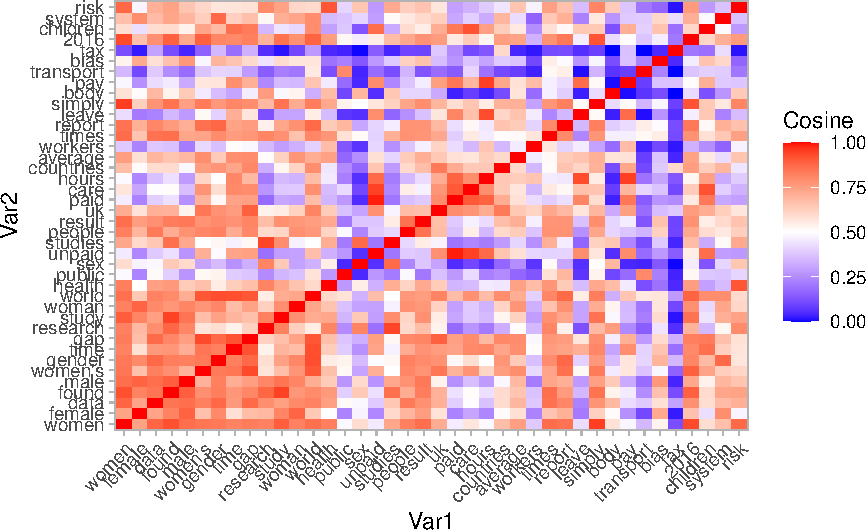
\includegraphics[width=0.7\linewidth]{report_files/figure-latex/euclidean similarities btwn words-1} \end{center}

\hypertarget{clustering-with-co-occurrences-uxe0-revoir}{%
\subsubsection{Clustering With Co-occurrences {[}à
revoir{]}}\label{clustering-with-co-occurrences-uxe0-revoir}}

Using co-occurrences to cluster features requires transforming
co-occurrences into dissimilarities. Object needs to be the tokens
because co-occurrences needs the token order and thus cannot be computed
on a BOW object.

Are terms co-occurring ? if yes, a lot ?

\begin{center}\includegraphics[width=0.7\linewidth]{report_files/figure-latex/clustering with co-occurrences-1} \end{center}

\begin{center}\includegraphics[width=0.7\linewidth]{report_files/figure-latex/clustering analysis-1} \end{center}

\hypertarget{topic-modeling}{%
\subsection{Topic Modeling}\label{topic-modeling}}

Topic modeling is a type of statistical modeling for discovering the
abstract ``topics'' that occur in a collection of documents. There are
two approaches: Latent Semantic Analysis model and Latent Dirichlet
Allocation model.

Both models can be applied on DTM or TF-IDF matrices.

\hypertarget{latent-semantic-analysis-lsa}{%
\subsubsection{Latent Semantic Analysis
(LSA)}\label{latent-semantic-analysis-lsa}}

\hypertarget{lsa-on-dtm}{%
\paragraph{LSA on DTM}\label{lsa-on-dtm}}

The Latent Semantic Analysis (LSA) is a dimension reduction method that
decomposes the DTM or TF-IDF matrices in three sub-matrices around a
pre-determined number of topics. Here, we proceed to LSA on the
document-term (i.e.~document-feature) matrix and then extract the
matrices of the LSA decomposition.

The first dimension of LSA is associated with the document lengths
(i.e.~sum of lines of DTM) this is why it is often ignored.

\hypertarget{topics-and-documents}{%
\subparagraph{Topics and Documents}\label{topics-and-documents}}

The below output shows the association between the first six chapters
and the ten topics. For example, text1 is associated the most with
dimension (i.e.~topic) 4 and the least associated with dimension
(i.e.~topic) 6.

\begin{verbatim}
#>          [,1]     [,2]     [,3]     [,4]     [,5]    [,6]      [,7]
#> text1  0.2018  0.11752 -0.19184  0.72710 -0.27103 -0.2251  0.476481
#> text2  0.1956  0.08192 -0.16037  0.42722 -0.09544  0.1764 -0.622684
#> text3  0.1485  0.04123 -0.12506  0.09144  0.26435  0.0798 -0.011243
#> text4  0.1923  0.07261 -0.11759 -0.02451  0.21483  0.8083  0.417789
#> text5  0.1302  0.03136  0.00308  0.05090  0.07383  0.1504 -0.208109
#> text6  0.1060  0.02393 -0.05058  0.07369  0.07692  0.1108 -0.189653
#> text7  0.0794  0.01738 -0.03277  0.05171  0.08908  0.0777 -0.079578
#> text8  0.0774  0.02957 -0.00125  0.00463  0.03408  0.0857  0.010204
#> text9  0.5744  0.58600  0.51451 -0.18195 -0.05804 -0.1336  0.018497
#> text10 0.5553 -0.73682  0.14966 -0.07018 -0.05705 -0.0955  0.073838
#> text11 0.2399 -0.23374  0.03162  0.02098  0.02088  0.0466 -0.096923
#> text12 0.0672  0.02220 -0.05154  0.07288  0.14703 -0.0243 -0.000291
#> text13 0.0951  0.04021 -0.13836  0.09835  0.84168 -0.3760  0.039819
#> text14 0.3172  0.16283 -0.76817 -0.45433 -0.20878 -0.1724  0.006966
#> text15 0.0293  0.00633 -0.02394  0.03464 -0.00029  0.0108 -0.040004
#> text16 0.1026  0.01312 -0.06164  0.08976  0.01562  0.0964 -0.326218
#>            [,8]     [,9]     [,10]
#> text1   0.08506  0.05690  0.039598
#> text2  -0.38771 -0.22719  0.076879
#> text3   0.24046  0.34038 -0.560136
#> text4  -0.20122 -0.10183  0.082302
#> text5   0.41032  0.47366  0.619532
#> text6   0.19092  0.28733 -0.000854
#> text7   0.69499 -0.69244 -0.007632
#> text8   0.06522  0.01795 -0.018213
#> text9  -0.05664 -0.03486 -0.025618
#> text10 -0.06282 -0.06250  0.147925
#> text11  0.04556  0.11108 -0.439631
#> text12  0.07124  0.05643 -0.103670
#> text13 -0.19409 -0.10575  0.173804
#> text14 -0.00778 -0.01062  0.039224
#> text15  0.00394 -0.00926 -0.027555
#> text16  0.00268  0.01373 -0.169465
\end{verbatim}

To verify if the first dimension is associated with the document length
we look at the below scatter-plot. We see that dimension 1 is negatively
correlated with the number ok tokens, which confirms that the first
dimension is associated with the document lenght.

{[}Improve plot: add a straight line showing the correlation{]}

\begin{center}\includegraphics[width=0.7\linewidth]{report_files/figure-latex/first dimension-1} \end{center}

\hypertarget{topics-and-features}{%
\subparagraph{Topics and Features}\label{topics-and-features}}

The below output shoes the association between the first six most
frequent words and the ten topics. For example, the term \emph{sexist}
is associated the most with topic 10.

\begin{verbatim}
#>               [,1]     [,2]      [,3]      [,4]      [,5]      [,6]
#> sexist     0.01200  0.00587 -0.019366 -0.000971 -0.000782  0.014755
#> joke       0.00810  0.00806  0.003833  0.006891 -0.004626 -0.005254
#> town       0.01863  0.01480 -0.007561  0.052847 -0.023678 -0.021740
#> karlskoga  0.01404  0.00898 -0.015193  0.061275 -0.025402 -0.021981
#> sweden     0.01626  0.00588 -0.021851  0.017419  0.005159 -0.000378
#> hit        0.00758 -0.00308 -0.002666  0.006217  0.002641  0.002664
#> initiative 0.00961  0.00607 -0.000971  0.007421  0.006773  0.006905
#> lens       0.00810  0.00806  0.003833  0.006891 -0.004626 -0.005254
#> harsh      0.00411  0.00218 -0.003676  0.008881 -0.000790  0.008543
#> glare      0.00281  0.00160 -0.002891  0.010112 -0.001743 -0.003654
#>                [,7]      [,8]      [,9]     [,10]
#> sexist      0.01335  0.010783 -0.014006  0.003486
#> joke        0.00758  0.000459  0.000367  0.000247
#> town        0.04406  0.007329  0.005101  0.003749
#> karlskoga   0.04864  0.009160  0.006312  0.004669
#> sweden     -0.01113  0.001419  0.010886 -0.027996
#> hit        -0.00826  0.002794  0.004926 -0.012127
#> initiative  0.00372  0.038046 -0.037837 -0.002577
#> lens        0.00758  0.000459  0.000367  0.000247
#> harsh       0.01369 -0.001876 -0.000748  0.002156
#> glare       0.00729  0.002525  0.001886 -0.001133
\end{verbatim}

To actually be able to interpret the topics (i.e.~dimensions) of the
LSA, we look at the ten terms with the largest values and the ten terms
with the lowest values. We take a look at dimension 4 and 5.

According to the below output, topic 4 is positively associated to
\emph{public}, \emph{transport}, \emph{sexual}, \emph{girls},
\emph{bus}, \emph{spaces}, \emph{data}, \emph{toilets},
\emph{harassment}, \emph{toilet} and negatively associated to
\emph{maternity}, \emph{drug}, \emph{heart}, \emph{pay}, \emph{trials},
\emph{paid}, \emph{hours}, \emph{sex}, \emph{unpaid}, \emph{leave}.
Therefore, documents that have a large dimension 4 use more these first
terms and less these last terms.

\begin{verbatim}
#>      transport     pedestrian            bus         travel 
#>         0.2744         0.2328         0.2146         0.1770 
#>           snow        sánchez      madariaga         toilet 
#>         0.1716         0.1716         0.1716         0.1474 
#>           trip             de       ambition             aw 
#>         0.1396         0.1381        -0.0689        -0.0919 
#>          dummy             mp     politician representation 
#>        -0.0920        -0.0924        -0.0971        -0.0977 
#>       election      candidate          party      interrupt 
#>        -0.0978        -0.1228        -0.1354        -0.1608
\end{verbatim}

According to the below output, topic 5 is positively associated to
\emph{female}, \emph{public}, \emph{trials}, \emph{politicians},
\emph{found}, \emph{representation}, \emph{party}, \emph{government},
\emph{political}, \emph{study} and negatively associated to
\emph{boler}, \emph{male}, \emph{motion}, \emph{seat}, \emph{vr},
\emph{dummy}, \emph{car}, \emph{body}, \emph{tech},
\emph{data}.Therefore, documents that have a large dimension 5 use more
these first terms and less these last terms.

\begin{verbatim}
#>        tax    poverty      marry     earner  household        pay 
#>     0.6936     0.1484     0.1167     0.1102     0.1100     0.1001 
#>     income       file     zombie     couple       trip         de 
#>     0.0970     0.0970     0.0947     0.0908    -0.0559    -0.0569 
#>     travel        bus       snow    sánchez  madariaga  interrupt 
#>    -0.0680    -0.0690    -0.0711    -0.0711    -0.0711    -0.0822 
#> pedestrian  transport 
#>    -0.0965    -0.1023
\end{verbatim}

\hypertarget{topics-and-documents-and-features}{%
\subparagraph{Topics and Documents and
Features}\label{topics-and-documents-and-features}}

The following biplot associates the positions of the terms (points) and
the positions of the document (arrows) in the LSA space for topics 4 and
5 computed above.

Here, we see that topic (i.e.~dimension) 4 is positively associated with
\emph{tech}, \emph{body}, \emph{data}, \emph{politicians},
\emph{female}, and anti-associated with \emph{transport}, \emph{leave},
\emph{sexy}.

\begin{center}\includegraphics[width=0.7\linewidth]{report_files/figure-latex/biplot2-1} \end{center}

\hypertarget{latent-dirichlet-allocation-lda}{%
\subsubsection{Latent Dirichlet Allocation
(LDA)}\label{latent-dirichlet-allocation-lda}}

The Latent Dirichlet Allocation is a generative model (i.e.~Bayesian
model) for topic modeling. LAD generates a Bag of Words model where the
number of topics are pre-defined.

The following output displays the ten most frequent terms per topic and
the ten most frequent topics per document.

\begin{verbatim}
#>       topic1       topic2     topic3        topic4     
#>  [1,] "public"     "stove"    "bias"        "worker"   
#>  [2,] "sexual"     "disaster" "hand"        "industry" 
#>  [3,] "toilet"     "woman"    "male"        "chemical" 
#>  [4,] "space"      "clean"    "student"     "body"     
#>  [5,] "girl"       "shelter"  "teach"       "violence" 
#>  [6,] "harassment" "violence" "algorithm"   "cancer"   
#>  [7,] "bus"        "country"  "hire"        "workplace"
#>  [8,] "official"   "report"   "voice"       "breast"   
#>  [9,] "report"     "plough"   "google"      "size"     
#> [10,] "crime"      "refugee"  "meritocracy" "pregnant" 
#>       topic5           topic6    topic7    topic8   topic9          
#>  [1,] "female"         "pay"     "sex"     "test"   "transport"     
#>  [2,] "government"     "unpaid"  "drug"    "car"    "travel"        
#>  [3,] "mp"             "hour"    "study"   "body"   "public"        
#>  [4,] "election"       "tax"     "trial"   "dummy"  "plan"          
#>  [5,] "party"          "country" "heart"   "crash"  "trip"          
#>  [6,] "politician"     "time"    "pain"    "seat"   "house"         
#>  [7,] "candidate"      "leave"   "medical" "tech"   "care"          
#>  [8,] "interrupt"      "care"    "disease" "vr"     "infrastructure"
#>  [9,] "parliament"     "child"   "body"    "design" "pedestrian"    
#> [10,] "representation" "uk"      "cell"    "motion" "home"          
#>       topic10 
#>  [1,] "woman" 
#>  [2,] "female"
#>  [3,] "datum" 
#>  [4,] "male"  
#>  [5,] "find"  
#>  [6,] "gender"
#>  [7,] "time"  
#>  [8,] "study" 
#>  [9,] "gap"   
#> [10,] "result"
\end{verbatim}

\begin{verbatim}
#>  [1] topic9  topic1  topic6  topic3  topic4  topic4  topic2  topic3 
#>  [9] topic8  topic7  topic7  topic6  topic6  topic5  topic10 topic2 
#> 10 Levels: topic1 topic2 topic3 topic4 topic5 topic6 ... topic10
\end{verbatim}

\hypertarget{term-topic-analysis}{%
\paragraph{Term-Topic Analysis}\label{term-topic-analysis}}

The term-topic analysis computes the conditional probability for a term
to be found given that it is assigned to a given topic. Then, for a
given topic, the largest conditional probabilities give the terms that
are the most associated with this topic.The advantage of LDA is that we
obtain the probabilities in addition to the term-topic assignment.

The below output shows for each ten topics, the terms with the highest
conditional probabilities. For example, this conditional probability for
the term \emph{women} is almost 1, indicating that \emph{women} is very
strongly associated with topic 5 and so that any document associated
with topic 5 will have the term \emph{women} in it. We also see that
some topics are better defined than others. For example, topic 5 is the
most well defined and topics 6, 7, 8 and 9 are not well defined.

To sum up, the tables below give the probabilities to select a term w
given that the term comes form topic k.

\begin{center}\includegraphics[width=0.7\linewidth]{report_files/figure-latex/term-topic-1} \end{center}

\hypertarget{topic-document-analysis}{%
\paragraph{Topic-Document Analysis}\label{topic-document-analysis}}

The topic-document analysis provided the probabilities for a topic to be
found in a document.

The below output shows that more than 60\% of topics 2 is about text 13
and more than 60\% of topic 3 is about text 14.

To dive a little bit deeper, we then look at the ten six longest
chapters (i.e.~documents).

\begin{verbatim}
#> [1] "text3"  "text9"  "text10" "text14" "text2"  "text4"
\end{verbatim}

{[}Improve layout: can we add chapter name instead of text ?{]}

Below we see that chapter 14 \emph{Women's Rights Are Human Rights}
mainly talks about topic 3.

\begin{center}\includegraphics[width=0.7\linewidth]{report_files/figure-latex/longest document plot-1} \end{center}

\hypertarget{lda-diagnosis}{%
\paragraph{LDA Diagnosis}\label{lda-diagnosis}}

The topic distribution (i.e.~proportion) in a corpus is called the topic
prevalence.

The following output displays the prevalence scores for each topic using
the thetas (i.e.~topic-document probabilities). Here, there are 16
documents. We see that the most prevalent topic is topic 5 with 0.3722.

\begin{verbatim}
#>  topic1  topic2  topic3  topic4  topic5  topic6  topic7  topic8 
#>  0.0580  0.0834  0.0665  0.0655  0.0407  0.1368  0.0714  0.0385 
#>  topic9 topic10 
#>  0.0477  0.3915
\end{verbatim}

\hypertarget{topic-modeling-measures}{%
\subsubsection{Topic Modeling Measures}\label{topic-modeling-measures}}

Topic modeling allows to organize, understand and summarize large
corpora (plural of corpus). Yet, topic modeling has limitations
especially regarding its interpretation of its outcomes. Therefore, some
measures provide a way to extract more insight from it.

\hypertarget{coherence}{%
\paragraph{Coherence}\label{coherence}}

The measure of coherence allows to assess the quality of a topic
(i.e.~good versus bad).

The below output gives the coherence for each ten topic. The most
coherent topic is topic 5 with a coherence of 0.428 and the least
coherent topic is topic 9 with a coherence of -8.934.

\begin{verbatim}
#>  [1] -3.969 -4.524 -5.741 -4.677 -8.080 -2.851 -4.306 -9.174 -3.742
#> [10]  0.557
\end{verbatim}

To verify we take a look at the co-document frequencies. Comparing the
two below term-frequency matrices for topic 9 and 4, it is obvious that
the top five terms in topic 5 are co-occurring more often in the same
document than the top five terms in topic 9.

\begin{verbatim}
#>             features
#> features     female government mp election party
#>   female         15         13  3        3     2
#>   government     13         13  3        3     2
#>   mp              3          3  2        3     2
#>   election        3          3  3        2     2
#>   party           2          2  2        2     2
\end{verbatim}

\begin{verbatim}
#>            features
#> features    transport travel public plan trip
#>   transport         2      3      4    5    2
#>   travel            3      4      5    4    2
#>   public            4      5      8    7    3
#>   plan              5      4      7    6    3
#>   trip              2      2      3    3    1
\end{verbatim}

\hypertarget{exclusivity}{%
\paragraph{Exclusivity}\label{exclusivity}}

A topic is exclusive if it is associated with terms that are not
associated to another topic.

The output below shows that the most exclusive topic (i.e.~topic which
as the more terms not associated with another topic) is topic 1 with an
exclusivity measure of 0.65252, meaning that its five top terms are more
specific to it, and the least exclusive one is topic 4 with 0.00280.

\begin{verbatim}
#>  [1] 0.75964 0.01084 0.01153 0.05086 0.00491 0.03552 0.00174 0.01656
#>  [9] 0.20167 0.02247
\end{verbatim}

\hypertarget{unsupervised-learning-embedding}{%
\subsection{Unsupervised learning:
Embedding}\label{unsupervised-learning-embedding}}

Embedding refers to the representation of elements (documents or tokens)
in a Vector Space Model (VSM).

\hypertarget{word-embedding-based-on-co-occurences-and-glove}{%
\subsubsection{Word Embedding Based on Co-occurences and
GloVe}\label{word-embedding-based-on-co-occurences-and-glove}}

The idea behind word embedding based on co-occurrences is to reflect
co-occurrences and not only Bag of Words (BoW).

To start with, we compute a feature co-occurrence symmetric matrix with
a window of five. The matrix is very large (8,640x8,640) and displays
the number of times terms (i.e.~features) appear together in a window of
five words.

\begin{verbatim}
#> Feature co-occurrence matrix of: 6 by 5,786 features.
#>            features
#> features    snow sexist joke town karlskoga sweden hit gender
#>   snow         0      3    1    2         3      1   0      6
#>   sexist       3      2    1    1         1      0   0      1
#>   joke         1      1    0    1         1      1   1      0
#>   town         2      1    1    0         1      1   1      3
#>   karlskoga    3      1    1    1         0      1   1      2
#>   sweden       1      0    1    1         1      0   1      1
#>            features
#> features    equality initiative
#>   snow             0          0
#>   sexist           0          0
#>   joke             0          0
#>   town             1          0
#>   karlskoga        1          1
#>   sweden           1          1
#> [ reached max_nfeat ... 5,776 more features ]
\end{verbatim}

From the feature co-occurrences matrix we compute two vector
representations for a given word (i.e.~feature). One representation for
a word being the central term and the other one for a word being in the
context. To then have a unique representation for a given word, we
compute the average of the two representations.

\begin{verbatim}
#> INFO  [18:31:32.809] epoch 1, loss 0.0352 
#> INFO  [18:31:32.873] epoch 2, loss 0.0278 
#> INFO  [18:31:32.912] epoch 3, loss 0.0249 
#> INFO  [18:31:32.945] epoch 4, loss 0.0230 
#> INFO  [18:31:32.977] epoch 5, loss 0.0218 
#> INFO  [18:31:33.009] epoch 6, loss 0.0211 
#> INFO  [18:31:33.041] epoch 7, loss 0.0206 
#> INFO  [18:31:33.072] epoch 8, loss 0.0202 
#> INFO  [18:31:33.105] epoch 9, loss 0.0200 
#> INFO  [18:31:33.137] epoch 10, loss 0.0197
\end{verbatim}

The following output displays the unique representations of the
vectors?.

\begin{verbatim}
#>              [,1]     [,2]
#> snow       -0.551 -0.14187
#> sexist     -0.647  0.10341
#> joke        0.259  0.06732
#> town        0.117 -0.24417
#> karlskoga   0.155 -0.50949
#> sweden     -0.370  0.00298
#> hit        -0.232  0.04333
#> gender     -2.503  1.55121
#> equality   -0.135 -0.32878
#> initiative  0.020  0.27665
\end{verbatim}

We now plot the vectors of the 50 most used words (50 largest
frequencies).

\begin{verbatim}
#>  [1] "woman"    "female"   "datum"    "male"     "find"    
#>  [6] "time"     "gender"   "women's"  "study"    "gap"     
#> [11] "sex"      "pay"      "report"   "research" "increase"
#> [16] "result"   "leave"    "design"   "country"  "include"
\end{verbatim}

\begin{center}\includegraphics[width=0.7\linewidth]{report_files/figure-latex/plot-1} \end{center}

\hypertarget{document-embedding}{%
\subsubsection{Document Embedding}\label{document-embedding}}

To build the document embedding we compute the centroids of the
documents. First, we need to extract the words in each document.

\begin{verbatim}
#> [1] "snow"     "clear"    "sexist"   "start"    "joke"     "official"
\end{verbatim}

Then, for these words we extract the word vectors and make a matrix.

\begin{verbatim}
#>            [,1]    [,2]
#> snow     -0.551 -0.1419
#> clear    -0.455 -0.1745
#> sexist   -0.647  0.1034
#> start    -1.078  0.9652
#> joke      0.259  0.0673
#> official -0.468  0.4844
\end{verbatim}

Finally, we average all these vectors.

\begin{verbatim}
#> [1] -0.395  0.540
\end{verbatim}

Now we make the loop to apply the previous steps on all documents.

\begin{verbatim}
#>         [,1]  [,2]
#> text1 -0.395 0.540
#> text2 -0.547 0.580
#> text3 -0.589 0.717
#> text4 -0.493 0.565
#> text5 -0.471 0.526
#> text6 -0.403 0.545
\end{verbatim}

\hypertarget{centroids-using-dtm}{%
\paragraph{Centroids using DTM}\label{centroids-using-dtm}}

\begin{center}\includegraphics[width=0.7\linewidth]{report_files/figure-latex/plot-texts-1} \end{center}

\hypertarget{centroids-using-tf-idf}{%
\paragraph{Centroids using TF-IDF}\label{centroids-using-tf-idf}}

\begin{center}\includegraphics[width=0.7\linewidth]{report_files/figure-latex/centroid plot tfidf-1} \end{center}

\hypertarget{supervised-analysis}{%
\subsection{Supervised Analysis}\label{supervised-analysis}}

The goal of the supervised analysis is to re-classify its documents
(i.e.~chapters) using the features (i.e.~terms) analyzed previously
{[}add where maybe{]} {[}is that a good reformulation of the aim?{]}. To
do so, we proceed to a machine learning approach consisting of splitting
the corpus (\emph{data} object) into a training and a test sets. Then,
we train the classifiers on the training set and finally the best
classifiers are selected on the test set.

To be able to proceed to the classification method described above, the
corpus must be cleaned in order for the features (i.e.~terms) to be
usable. The cleaning process is achieved in the \emph{Data Structuring
and Cleaning} of the \textbf{Data} section and consists in sequential
steps from the tokenization, removing useless words (i.e.~stop words),
lemmatization (i.e.~tokens simplification) to stemming (i.e.~reduce
words to their stems).

\begin{verbatim}
#> Confusion Matrix and Statistics
#> 
#>           Reference
#> Prediction  1  2  3  4  5  6
#>          1 18  1  1  1  1  2
#>          2  2 30  2  6 10  2
#>          3  1  8 19  3  4  0
#>          4  0  0  0 14  0  0
#>          5  0  2  2  1 16  0
#>          6  1  0  0  0  2  5
#> 
#> Overall Statistics
#>                                         
#>                Accuracy : 0.662         
#>                  95% CI : (0.582, 0.736)
#>     No Information Rate : 0.266         
#>     P-Value [Acc > NIR] : <2e-16        
#>                                         
#>                   Kappa : 0.581         
#>                                         
#>  Mcnemar's Test P-Value : NA            
#> 
#> Statistics by Class:
#> 
#>                      Class: 1 Class: 2 Class: 3 Class: 4 Class: 5
#> Sensitivity             0.818    0.732    0.792   0.5600    0.485
#> Specificity             0.955    0.805    0.877   1.0000    0.959
#> Pos Pred Value          0.750    0.577    0.543   1.0000    0.762
#> Neg Pred Value          0.969    0.892    0.958   0.9214    0.872
#> Prevalence              0.143    0.266    0.156   0.1623    0.214
#> Detection Rate          0.117    0.195    0.123   0.0909    0.104
#> Detection Prevalence    0.156    0.338    0.227   0.0909    0.136
#> Balanced Accuracy       0.886    0.769    0.834   0.7800    0.722
#>                      Class: 6
#> Sensitivity            0.5556
#> Specificity            0.9793
#> Pos Pred Value         0.6250
#> Neg Pred Value         0.9726
#> Prevalence             0.0584
#> Detection Rate         0.0325
#> Detection Prevalence   0.0519
#> Balanced Accuracy      0.7674
\end{verbatim}

\begin{verbatim}
#> Random Forest 
#> 
#> 102 samples
#>  30 predictor
#>   6 classes: '1', '2', '3', '4', '5', '6' 
#> 
#> Pre-processing: centered (30), scaled (30) 
#> Resampling: Bootstrapped (25 reps) 
#> Summary of sample sizes: 102, 102, 102, 102, 102, 102, ... 
#> Resampling results across tuning parameters:
#> 
#>   mtry  splitrule   Accuracy  Kappa
#>    2    gini        0.558     0.440
#>    2    extratrees  0.542     0.416
#>    5    gini        0.575     0.461
#>    5    extratrees  0.573     0.457
#>    8    gini        0.566     0.452
#>    8    extratrees  0.590     0.482
#>   11    gini        0.565     0.451
#>   11    extratrees  0.596     0.488
#>   14    gini        0.560     0.446
#>   14    extratrees  0.595     0.489
#>   17    gini        0.560     0.447
#>   17    extratrees  0.583     0.472
#>   20    gini        0.551     0.436
#>   20    extratrees  0.595     0.489
#>   23    gini        0.555     0.440
#>   23    extratrees  0.604     0.501
#>   26    gini        0.545     0.430
#>   26    extratrees  0.590     0.481
#>   30    gini        0.537     0.421
#>   30    extratrees  0.601     0.496
#> 
#> Tuning parameter 'min.node.size' was held constant at a value of 1
#> Accuracy was used to select the optimal model using the
#>  largest value.
#> The final values used for the model were mtry = 23, splitrule
#>  = extratrees and min.node.size = 1.
\end{verbatim}

\hypertarget{conclusion}{%
\section{Conclusion}\label{conclusion}}

\begin{itemize}
\tightlist
\item
  Take home message
\item
  Limitations
\item
  Future work?
\end{itemize}

\end{document}
